\documentclass[conference]{IEEEtran}
\IEEEoverridecommandlockouts
% The preceding line is only needed to identify funding in the first footnote. If that is unneeded, please comment it out.
%Template version as of 6/27/2024
\usepackage{stmaryrd}
\usepackage{hyperref}
% \hypersetup{colorlinks=true,citecolor = blue}
\newcommand{\Spt}{\texttt{Spt}}
\newcommand{\Rec}{\texttt{Rec}}
\newcommand{\DEnc}{\texttt{DEnc}}
\newcommand{\PEnc}{\texttt{PEnc}}
\usepackage[ruled,vlined,linesnumbered]{algorithm2e}
\usepackage{algorithmic}
\usepackage{booktabs}
\usepackage{multirow}
\usepackage{subfigure}
\usepackage{changepage}
\usepackage{cite}
\usepackage{amsmath,amssymb,amsfonts}
\usepackage{graphicx}
\usepackage{textcomp}
\usepackage{xcolor}
\def\BibTeX{{\rm B\kern-.05em{\sc i\kern-.025em b}\kern-.08em
    T\kern-.1667em\lower.7ex\hbox{E}\kern-.125emX}}
\begin{document}

\title{MIND: A Privacy-Preserving Model Inference Framework via End-Cloud Collaboration
% *\\
% {\footnotesize \textsuperscript{*}Note: Sub-titles are not captured for https://ieeexplore.ieee.org  and
% should not be used}
% \thanks{Identify applicable funding agency here. If none, delete this.}
}

% \author{\IEEEauthorblockN{1\textsuperscript{st} Siyuan Guan}
% \IEEEauthorblockA{\textit{Guangzhou Institute of} \\
% \textit{Technology, Xidian University}\\
% Guangzhou, China \\
% siyuanguan@stu.xidian.edu.cn}
% \and
% \IEEEauthorblockN{2\textsuperscript{nd} Ziheng Hu}
% \IEEEauthorblockA{\textit{Guangzhou Institute of} \\
% \textit{Technology, Xidian University}\\
% Guangzhou, China \\
% 649704937hu@gmail.com}
% \and
% \IEEEauthorblockN{3\textsuperscript{rd} Guotao Xu}
% \IEEEauthorblockA{\textit{Guangzhou Institute of} \\
% \textit{Technology, Xidian University}\\
% Guangzhou, China \\
% guotaoxu@stu.xidian.edu.cn}\\
% \and
% \IEEEauthorblockN{4\textsuperscript{th} Yao Zhu}
% \IEEEauthorblockA{\textit{Guangzhou Institute of} \\
% \textit{Technology, Xidian University}\\
% Guangzhou, China \\
% 22151214570@stu.xidian.edu.cn}
% \and
% \IEEEauthorblockN{5\textsuperscript{th} Bowen Zhao*}
% \IEEEauthorblockA{\textit{Guangzhou Institute of} \\
% \textit{Technology, Xidian University}\\
% Guangzhou, China \\
% bwinzhao@gmail.com}
% \and
% \IEEEauthorblockN{6\textsuperscript{th} Given Name Surname}
% \IEEEauthorblockA{\textit{dept. name of organization (of Aff.)} \\
% \textit{name of organization (of Aff.)}\\
% City, Country \\
% email address or ORCID}
% }
\author{
\IEEEauthorblockN{1\textsuperscript{st} Siyuan Guan}
\IEEEauthorblockA{\textit{Guangzhou Institute of} \\
\textit{Technology, Xidian University}\\
Guangzhou, China \\
siyuanguan@stu.xidian.edu.cn}
\and
\IEEEauthorblockN{2\textsuperscript{nd} Ziheng Hu}
\IEEEauthorblockA{\textit{Guangzhou Institute of} \\
\textit{Technology, Xidian University}\\
Guangzhou, China \\
649704937hu@gmail.com}
\and
\IEEEauthorblockN{3\textsuperscript{rd} Guotao Xu}
\IEEEauthorblockA{\textit{Guangzhou Institute of} \\
\textit{Technology, Xidian University}\\
Guangzhou, China \\
guotaoxu@stu.xidian.edu.cn}
\and
\hspace{4cm}\IEEEauthorblockN{4\textsuperscript{th} Yao Zhu}
\IEEEauthorblockA{\hspace{4cm}\textit{Guangzhou Institute of} \\
\hspace{4cm}\textit{Technology, Xidian University}\\
\hspace{4cm}Guangzhou, China \\
\hspace{4cm}22151214570@stu.xidian.edu.cn}
\and
\IEEEauthorblockN{5\textsuperscript{th} Bowen Zhao*}
\IEEEauthorblockA{\textit{Guangzhou Institute of} \\
\textit{Technology, Xidian University}\\
Guangzhou, China \\
bwinzhao@gmail.com}
\and
}

\maketitle

\begin{abstract}
Image processing and analysis capabilities have been revolutionized by the rapid advancement of deep learning technologies. Model inference enables powerful image analytics, however, complex neural networks often require more computing and storage resources than end devices can provide. While Cloud-based model inference helps alleviate the resource constraints of these devices. However, transferring sensitive image data to the cloud server arises significant privacy concerns. Existing approaches usually either encrypt the images locally and send them to the cloud server or deploy the model locally, which fails to exploit the computing capability of the end devices or reveals machine learning model. To this end, in this paper, we proposed MIND, a privacy-preserving model inference framework via end-cloud collaboration. MIND makes the end devices and the cloud server jointly perform layer-by-layer computations required by model inference through cryptographic primitives including the homomorphic cryptosystem and additive secret sharing. For linear layers, MIND always chooses the less expensive option between data encryption and model parameters encryption. 
Results of experimental evaluations on several models show MIND  effective and outperforms the existing solutions.
\end{abstract}

\begin{IEEEkeywords}
Homomorphic encryption, secret sharing, model inference, privacy protection.
\end{IEEEkeywords}

\section{Introduction}
Advancements in artificial intelligence and cloud computing have revolutionized image processing and analysis across various industries \cite{makridakis2017forthcoming} \cite{zhang2010cloud}. Model inference has become a critical component in cloud-based image processing and analysis, leveraging deep learning models to extract valuable insights from visual data. This approach enables sophisticated image interpretation across various domains, from medical diagnostics to autonomous systems. However, the widespread adoption of cloud-based model inference has raised significant privacy concerns, as it often requires the transmission and processing of sensitive personal data \cite{shokri2017membership}\cite{wang2018stealing}. For instance, facial recognition systems in residential areas and financial institutions' use of image data for commercial purposes exemplify scenarios where user privacy may be compromised \cite{cui2018security}. These practices highlight the tension between leveraging advanced technologies and protecting individual privacy rights.

Conventionally, image analysis involves encrypting the entire image before uploading it to the cloud. However, this approach leads to substantial storage and communication overhead due to the size of encrypted images. Additionally, conducting image analysis during transmission poses significant privacy challenges, as sensitive data must be securely handled to prevent unauthorized access \cite{van2014datafication}.

Existing privacy-preserving schemes for model inference attempt to address these concerns through various encryption techniques \cite{fu2020vfl}\cite{yang2012efficient}. Traditional encryption methods, while providing a degree of data security, often introduce substantial computational overhead and communication cost \cite{kerschbaum2012outsourced}. This inefficiency becomes particularly pronounced when dealing with large-scale data, which hinders the practicality of such approaches in real-world scenarios \cite{li2015encdb}. Moreover, current solutions struggle to balance privacy protection, computational efficiency, and communication overhead, especially in end-to-cloud collaborative environments.
% \subsection{Contribution}

To address these limitations, we propose MIND, a novel privacy-preserving model inference framework enabled by end-to-cloud collaboration. MIND integrates advanced technologies such as homomorphic encryption and secret sharing to secure both data and model parameters throughout the inference process. By distributing computational tasks between end devices and cloud servers, MIND enhances data privacy, reduces communication overhead, and maintains inference efficiency. A key feature of MIND is its layered encryption scheme, which dynamically adjusts encryption methods based on the model structure, optimizing computational and communication costs. The main contributions of our work are summarized as follows:

\begin{itemize}
    \item We propose a novel privacy-preserving model inference framework via end-cloud collaboration, named MIND\footnote{MIND: a privacy-preserving \underline{m}odel \underline{i}nference framework via a\underline{n}d-clou\underline{d} collaboration}. MIND incorporates secret sharing and homomorphic encryption to safeguard sensitive information in both data and models. Additionally, MIND enables collaborative computations between cloud server while ensuring that privacy is not compromised.
    
    \item We present a novel method that employs hierarchical encryption, which introduces a layered approach using both data and parameter encryption. MIND overcomes the limitations of existing solutions while maintaining the original recognition accuracy.
    
    \item We conduct extensive experiments on MNIST to demonstrate the effectiveness and efficiency of MIND. Experimental evaluations show that MIND outperforms the existing solution in terms of communication cost and runtime.  
%第三点还需要修改    
\end{itemize}
\section{Related work}
As the demand for secure data processing in cloud computing environments increases, researchers have conducted various studies to improve the efficiency and privacy protection of collaborative inference methods between cloud servers and end devices. To address these challenges, researchers have proposed numerous solutions based on various technologies. We categorize previous work into three main subcategories.

Federated learning (FL) is an innovative approach to machine learning that prioritizes the privacy of training data. In horizontal FL (e.g., \cite{pmlr-v54-mcmahan17a}, \cite{Gupta2018DistributedLO}, \cite{9252066}), each client (i.e., data owner or end devices) independently trains a local model using its private data and then submits the obfuscated local models to a central model aggregator (i.e., model owner or cloud server). However, because the global model is synchronized during each training iteration, FL does not adequately address the privacy related to the global model. Furthermore, FL tends to disproportionately favor end devices, as each end device gains access to the global model even if they contribute only a small portion of the training data. Consequently, when the server has an exclusive proprietary interest in the final model, FL is not an ideal solution.

To safeguard both data and model privacy, the research community has developed a range of distributed training methods centered on secure multiparty computation (MPC, e.g., \cite{7958569}, \cite{Escudero2020ImprovedPF}, \cite{Dalskov2020FantasticFH}). In these approaches, the typical scenario involves a server-assisted framework where a group of data owners uploads secret-shared versions of their private data to at least two independent, non-colluding third-party servers. These servers collaboratively train the model using the secret-shared data. During the training process, the model itself is also secret-shared across all servers, ensuring complete protection of model privacy. However, as previously mentioned, these approaches face a significant trade-off between the requirements for non-collusion and the need for extensibility.

The third subcategory of research depends on homomorphic encryption (HE, e.g, \cite{Nandakumar2019TowardsDN,CiC-1-2-22,9888863,zhao2023identifiable}). In cloud computing \cite{gentry2009fully}, which allows computations to be performed on encrypted data without the need for decryption. This approach makes it feasible to execute complex operations on cloud servers while maintaining data privacy. However, the computational overhead associated with fully homomorphic encryption remains non-trivial when dealing with large-scale data \cite{xu2019cryptonn}. Although Cheon \textit{et al.} \cite{cheon2017homomorphic} have attempted to optimize homomorphic encryption scheme to reduce this overhead, the trade-off between computational efficiency and security continues to be a critical issue.

As research progresses, there is a growing interest in leveraging the strengths of both edge and cloud computing to enhance security and efficiency. To leverage the advantages of both approaches, Mao \textit{et al.} \cite{mao2017survey} proposed an end-cloud collaborative model. While this approach shows promise, it imposes certain performance requirements on the end devices and does not effectively address the issue of reducing communication overhead. In a related effort, Akshaya and Khadir \textit{et al.} \cite{kakkad2019biometric} explored approaches to enhance image security in cloud frameworks using biometric authentication and image encryption.

% In summary, the traditional encryption methods for collaborative inference between cloud server and terminals typically involve directly encrypting image data. While this approach can protect data privacy, it has certain limitations in terms of computational efficiency and communication overhead. The end-cloud collaboration has proven to be a promising approach for privacy-preserving data processing, with various models and techniques contributing to its development.  The MIND framework advances this field by addressing the limitations of existing methods and offering a efficient and secure solution for model inference in cloud computing environments.

\section{Preliminaries}
This section provides some preliminaries of MIND, with a particular focus on homomorphic encryption and additive secret sharing.
\begin{table}[h]
\centering
\caption{Notations}
\label{table:notations}
\begin{tabular}{c|c}
\toprule
\textbf{Notations} & \textbf{Description} \\ 
\midrule
$pk_e$                                   & Public key of the end devices. \\
$pk_s$                                   & Public key of the cloud servers. \\
$sk_e$                                   & Private key of the end devices. \\
$sk_s$                                   & Private key of the cloud servers. \\
$\llbracket \cdot \rrbracket_{pk_e}$     & Ciphertext encrypted using the public key $pk_e$. \\
$\llbracket \cdot \rrbracket_{pk_s}$     & Ciphertext encrypted using the public key $pk_s$. \\
$\langle \cdot \rangle_i$                & Secret share between $ED$ and $S$. \\
$r_j$                                    & Random vector generated by 
$ED$ and $S$. \\
% $w_p$                                    & The model weights of parametric encryption (\PEnc).\\
% $w_d$                                    & The model weights of data encryption (\DEnc).\\
$w_j$                                      & Weights of the model in layer $j$. \\
$b_j$                                      & Bias parameters of the model in layer $j$. \\
% \multirow{2}{*}{$y_p$}                                    & The intermediate computed result after the encryption \\
%                                               & of model parameters on the end devices.\\
$y_j$                                    & Computation result after encryption in layer $j$.\\
$N_{p}$          & Number of bits representing the model parameters..\\
$N_{d}$          & Number of bits representing the model data.\\
\circ            & Linear operator.\\
\multirow{2}{*}{\oplus}           & Addition operation for two \\                                       & encrypted values in the HE scheme.\\
\multirow{2}{*}{\ominus}          & Denotes the subtraction of two\\  
                                  & encrypted values in the HE scheme.\\
\multirow{2}{*}{\otimes}          & Denotes the multiplication of two\\
                                  & encrypted values in the HE scheme.\\
\bottomrule
\end{tabular}
\end{table}

\subsection{Homomorphic Encryption}\label{HE}
In this work, we consider the BFV-level homomorphic encryption homomorphic encryption cryptosystem, which is based on the Ring-Learning With Errors (RLWE) problem with residual number system (RNS) optimization \cite{bajard2016full}. Specifically, the BFV scheme takes a set of parameters $\{N, t, q\}$ as input, where $N$ represents the polynomial degree with a power of two, and $t$, $q$ denote the modulus of the plaintext and the ciphertext, respectively. $\mathcal{R}_{t,N} = \mathbb{Z}_t [X]/(X^N + 1)$ is the polynomial ring that denotes the plaintext space, and $\mathcal{R}_{q, N}^2$ defines the ciphertext space.

The BFV scheme based on RLWE supports additive homomorphism and multiplication homomorphism. Given two ciphertexts $\llbracket x \rrbracket_{pk}$ and $\llbracket y \rrbracket_{pk}$ encrypted with public key $pk$, the addition $\oplus$ (also subtraction $\ominus$) and multiplication $\otimes$ of polynomials in the encrypted domain are formulated in the following:
\begin{equation*}
\begin{array}{c}
    \llbracket x \rrbracket_{pk} \oplus \llbracket y \rrbracket_{pk} = \llbracket x + y \rrbracket_{pk}. \\
    \llbracket x \rrbracket_{pk} \otimes \llbracket y \rrbracket_{pk} = \llbracket x \times y \rrbracket_{pk}.    
\end{array}
\end{equation*}

\subsection{Secret Sharing}\label{SS}
We utilize an additive secret sharing scheme upon the ring $\mathbb{Z}_t$ (integers modulo $t$) with $t = 2^\lambda$, which comprises a split function and a recovery function in the following:
\begin{itemize}
\item \textbf{Split} (\Spt): \texttt{Spt} takes an origin secret $x \in \mathbb{Z}_t$ as input and outputs two secret shares $\langle x \rangle_1 \in \mathbb{Z}_t$ and $\langle x \rangle_2 \in \mathbb{Z}_t$, denoted as
\begin{equation}
    (\langle x \rangle_1, \langle x \rangle_2) \gets \Spt(x) = (r, x - r\!\!\!\mod t),
\end{equation}
where $r$ is a randomly chosen from $\mathbb{Z}_t$.

\item \textbf{Recovery} (\Rec): \texttt{Rec} takes two secret shares $\langle x \rangle_1 \in \mathbb{Z}_t$ and $\langle x \rangle_2 \in \mathbb{Z}_t$, and outputs the origin secret $x \in \mathbb{Z}_t$, formulated as
\begin{equation}
     x \gets \Rec(\langle x \rangle_1, \langle x \rangle_2) = \langle x \rangle_1 + \langle x \rangle_2\!\!\!\mod t.
\end{equation}
\end{itemize}

Considering the BFV scheme and integer-based secret sharing, input data may involve decimal numbers rather than integers. The work \cite{liu2024pencilprivateextensiblecollaborative,8611203} convert decimal numbers to integers. In this work, we adopt a fixed-point representation of decimal numbers with a precision of $\ell$ bits, formulated as $x \gets \lfloor \tilde{x} \cdot 2^\ell \rfloor \in \mathbb{Z}$, where $\tilde{x} \in \mathbb{R}$. To avoid overflow, truncation is required after each multiplication operation, and all intermediate results must not exceed $\pm t/2^{2\ell + 1}$ in their decimal form.

\subsection{Forward Propagation in Neural Networks}

In neural network inference, forward propagation refers to the process of passing input data through each layer of the network to obtain the final output. For linear layers, this process can be abstracted by the equation:
\begin{equation*}
\begin{array}{c}
       y=f(x)=f(x;W,b)=W\circ x+b
\end{array}
\end{equation*}
Here, $W$ denotes the weight matrix, $x$ represents the input vector, and $b$ is the bias vector. The operator $\circ$ is a linear operator that satisfies the distributive property:
\begin{equation*}
% \begin{array}{c}
       (u_0+u_1) \circ (v_0+v_1)=u_0 \circ v_0+u_1 \circ v_0+ u_0\circ v_1+ u_1\circ v_1
% \end{array}
\end{equation*}

In different types of layers, this operator $\circ$ takes on different meanings. In fully connected layers, $\circ$ represents matrix-vector multiplication, defined as $y=W·x+b$, where $W$ is a matrix and $x$ is a vector. In 2-dimensional convolution layers, $\circ$ represents the convolution operation, expressed as $W\circ x=\text{Conv}2\text{d}(x;W)$, where the convolution operation is applied between the input $x$ and the weight $W$ to produce the output.

\section{Formulation}
In this section, we formalize the system model, threat model, and security objectives. The system model specifies the entities involved and their capabilities. The threat model identifies the adversary's potential attack strategies. Finally, the security objectives define the protections required to mitigate these threats effectively.
\subsection{System Model}
 In MIND, we propose an end-cloud collaborative privacy-preserving inference framework, as illustrated in Fig. \ref{fig:system_model}. The framework comprises two key entities: the End Device ($ED$) and the Cloud Server ($S$). The roles and functions of each entity are detailed below. The notations used throughout this work are summarized in Table \ref{table:notations}.
\begin{figure}[ht]
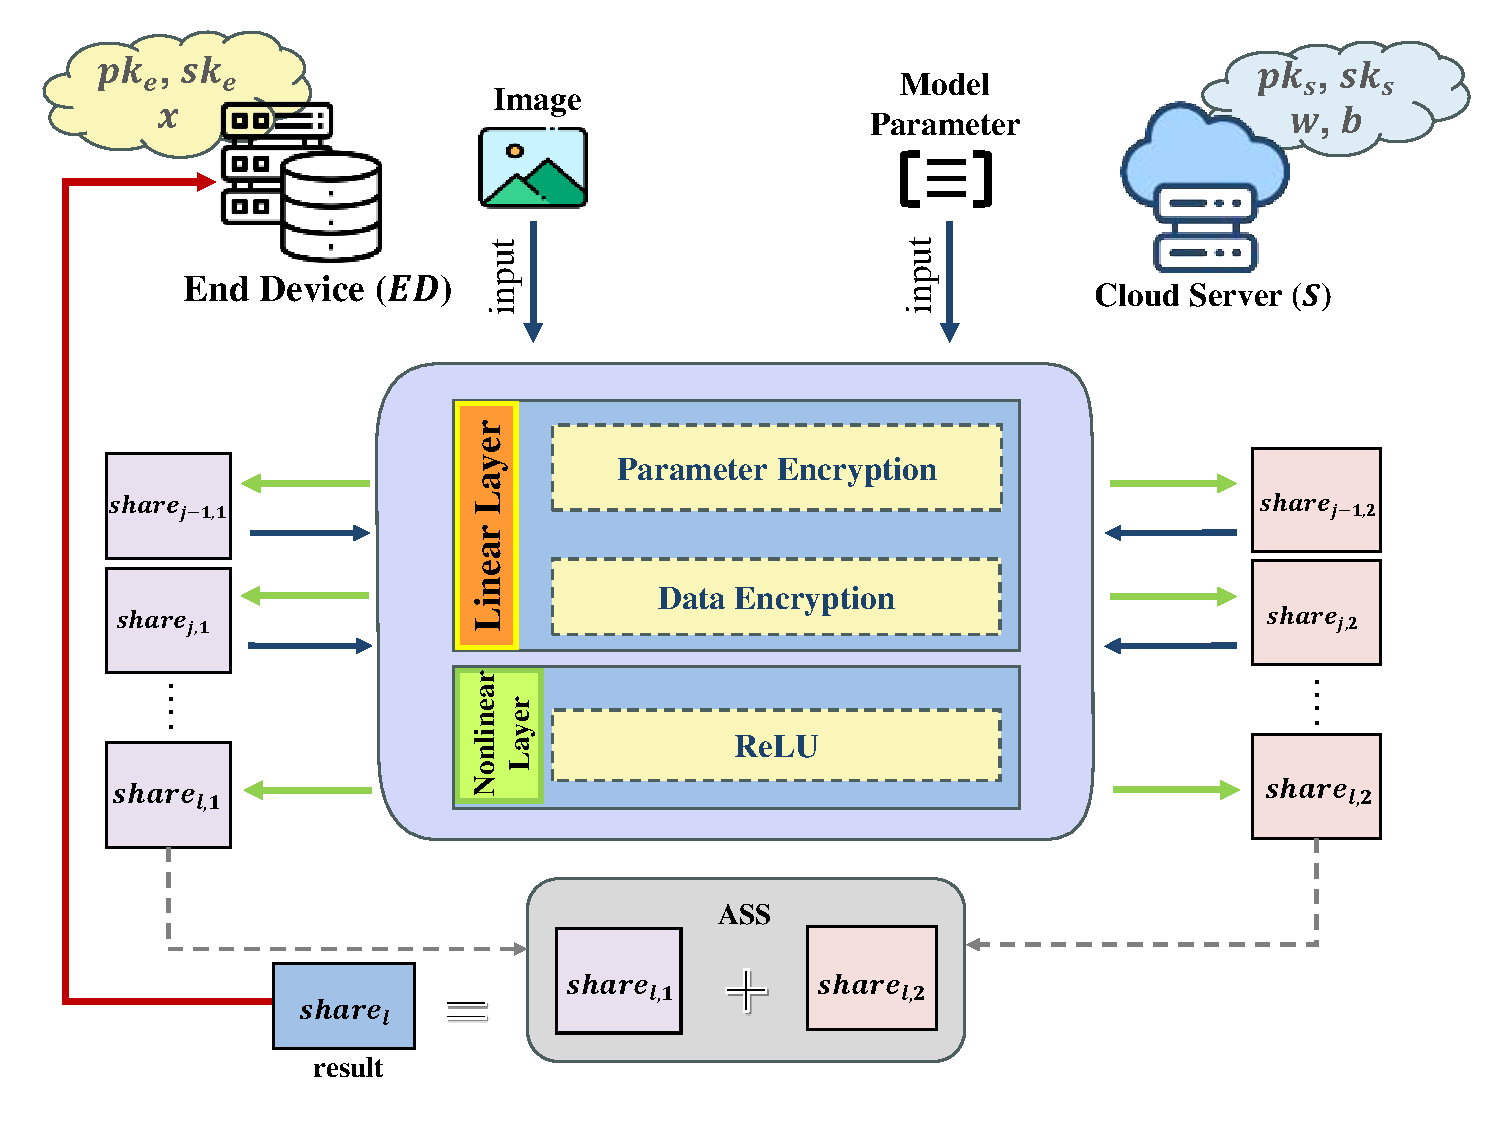
\includegraphics[width=1\linewidth]{fig1.pdf}
\caption{System model.} \label{fig:system_model}
\end{figure}

$ED$: The end device ($ED$) serves as the image data owner. $ED$ holds the architecture of a deep learning model along with a set of public and private keys ($pk_e,sk_e$). $ED$ performs iterative computations by interacting with the cloud server using homomorphic encryption and secret splitting. Finally, $ED$ combines the secret shares received from the cloud server and local endpoints to derive inference results.

$S$: The cloud server ($S$) acts as an auxiliary computing entity. $S$ stores the parameters of the deep learning model and maintains a set of public and private keys ($pk_s,sk_s$). $S$ engages in iterative computations by interacting with the endpoints through homomorphic encryption and secret splitting. Finally, $S$ sends its secret share of the computations to $ED$.

%  TODO: 下面这段话应该放到后面
%  This architecture ensures both security and efficiency in face recognition processes by distributing computational tasks and securely handling sensitive data. Moreover, it leverages advanced cryptographic techniques to protect data privacy throughout the entire workflow.	

\subsection{Threat Model and Security Goal}
In our system, the main threats include: attackers intercepting and tampering with image data, model parameters, or computation results transmitted between the $ED$ and $S$, leading to unauthorized access or data manipulation; the cloud server, or a compromised part of it, analyzing shared data to infer the original image or its features, thereby violating user privacy; and attackers targeting the $ED$ or cloud server to gain access to raw or secretly shared data, compromising the security of the entire system. Based on the above threat model, our security goals are listed as follows:
\begin{itemize}
     \item \textit{Data integrity and confidentiality}: Before transmitting images to $S$ or sending model parameters to $ED$, the data is encrypted using a public key. During the computation process, a combination of homomorphic encryption and additive secret sharing (e.g., $\langle x \rangle_1$ and $\langle x \rangle_2$) is employed. This ensures that no single server possesses sufficient information to reconstruct the original data. These measures safeguard the image and its features from exposure to unauthorized parties during transmission and storage. Additionally, they ensure the integrity of the data exchanged between $ED$ and $S$, preventing tampering during transit. 
     \item \textit{Collusion Resistance}: Ensure that only authorized entities $ED$ and $S$ can access and process encrypted feature vectors, preventing unauthorized inference of biometric information. If one of the servers is compromised or colludes with an attacker, they cannot reconstruct the original feature vectors without the shares from the other server.
 \end{itemize}
 
\section{MIND Design}
In this section, we first detail the hierarchical cryptographic inference algorithm designed for the linear layer of the model, followed by describing the design of the algorithm for the nonlinear layer, and finally explaining the whole inference process. Table \ref{table:notations} summarizes the notation used in this paper.
% \subsection{Scheme Construction}
% 详细解释系统如何实现加法秘密共享和同态加密,包括技术细节和算法。

% \subsection{Secret sharing of image features}
% % In MIND, multiple organizations collaborate on tasks related to model training and data interaction. The data owned by these organizations are temporary and cannot be directly shared. It is assumed that all institutions involved in the training process are rigorously verified as non-malicious participants, ensuring they do not engage in activities such as poisoning attacks that could compromise the model or the training process.

% As shown in Fig. \ref{fig:system_model}, $ED$ plays a dual role in this system. It is both a data receiver and a sender. As an end device, $ED$ first collects images. It then uses a local feature extraction model to extract feature vector. Fig. \ref{fig:ED_Models} shows the detailed data processing flow. To ensure data security, $ED$ uses additive secret sharing to securely split the feature vector. After extracting the feature vector from the collected image, $ED$ first generates an $n$-dimensional random vector $\langle x \rangle_1$, with each element randomly selected from $\mathbb{Z}_t$. $ED$ then creates a second share $\langle x \rangle_2$, by subtracting this random vector $\langle x \rangle_1$ from the original feature vector $v$. This process is represented by the following formula:
% $\langle x \rangle_2 = v - \langle x \rangle_1$
% The sum of share $\langle x \rangle_1$ and share $\langle x \rangle_2$ equals the original feature vector $v$. This design protects the privacy of feature information. It also enables secure distributed storage. Even when data is split and stored in a distributed manner, it can be securely reconstructed. This mechanism greatly enhances the system's security and privacy protection. At the same time, it maintains data usability and integrity.


\subsection{Encrypted Inference for Linear Layers }
Traditional encryption methods for collaborative inference between cloud servers and end devices often encrypt image data directly. Although this approach protects data privacy, it has limitations in terms of computational efficiency and communication overhead. To address these issues, we propose MIND, a novel end-cloud collaborative encryption method. This new approach divides the encryption process into two parts: model parameter encryption and image data encryption. As shown in Figure\ref{fig:MIND Overview} ,our method applies these two encryption techniques to different linear network layers. This division allows for a more efficient and flexible approach to data protection.

In the \PEnc~algorithm (Algorithm \ref{alg:Parameter}), the inputs include $\langle x_{j-1}\rangle_1$ and $\langle x_{j-1}\rangle_2$ as the feature vector to be encryted, the weight $w_{j-1}$, and the bias $b_{j-1}$. Specifically, $ED$ holds $\langle x_{j-1}\rangle_1$, while $S$ holds $\langle x_{j-1}\rangle_2$, $w_{j-1}$ and $b_{j-1}$. As described in \PEnc~, $S$ encrypts the model weights $w_{j-1}$ using the public key $pk_s$ and transmitting the encrypted weights $\llbracket w_{j-1} \rrbracket_{pk_s}$ to $ED$. Upon receiving $\llbracket w_{j-1} \rrbracket_{pk_s}$, $ED$ performs a homomorphic multiplication operation to evaluate the product of $\llbracket w_{j-1} \rrbracket_{pk_s}$ and $\langle x_{j-1} \rangle_1$, yielding the result $\llbracket w_{j-1} \langle x_{j-1} \rangle_1\rrbracket_{pk_s} = \llbracket w_{j-1} \times \langle x_{j-1} \rangle_1 \rrbracket_{pk_s}$. Subsequently, $ED$ introduces a random number $r_{j-1}\in \mathbb{Z}_t$ and calculates the encrypted result $\llbracket C \rrbracket_{pk_s}=\llbracket w_{j-1} \langle x_{j-1} \rangle_1 + r_{j-1} \rrbracket_{pk_s}$, which is then sent back to $S$. $S$ decrypts $\llbracket C \rrbracket_{pk_s}$ to retrieve the value $w_{j-1}\langle x_{j-1} \rangle_1+r_{j-1}$. Next, $S$ calculates the result $\langle y_j\rangle_2= w_{j-1}(\langle x_{j-1} \rangle_1 + \langle x_{j-1} \rangle_2)+r_{j-1}+b_{j-1}=w_{j-1}x+r_{j-1}+b_{j-1}$, $ED$ obtains the result $\langle y_j\rangle_1=-r_{j-1}$. 
\begin{algorithm}[htbp]
	\caption{\PEnc$(\langle x_{j-1} \rangle_1,\langle x_{j-1} \rangle_2,w_{j-1},b_{j-1}) \rightarrow (\langle y_j\rangle_1, \langle y_j\rangle_2)$}
    \label{alg:Parameter}
    \LinesNumbered
	\KwIn{$ED$ holds $\langle x_{j-1} \rangle_1$. \\
	\hspace{33pt}$S$ holds $\langle x_{j-1} \rangle_2$, $w_{j-1}$, and $b_{j-1}$.}
    \KwOut {Secret shares $\langle y_j \rangle_1 $ and $\langle y_j \rangle_2$.}
     $S$ sends $\llbracket w_{j-1}\rrbracket_{pk_s}$ to $ED$;
    
     $ED$ evaluates $\llbracket w_{j-1}\langle x_{j-1} \rangle_1 \rrbracket_{pk_s} = \llbracket w_{j-1} \rrbracket_{pk_s} \otimes \llbracket \langle x_{j-1} \rangle_1 \rrbracket_{pk_s}$;
    
     $ED$  calculates $\llbracket C\rrbracket_{pk_s} = \llbracket w_{j-1}\langle x_{j-1} \rangle_1 \rrbracket_{pk_s} \oplus \llbracket r_{j-1} \rrbracket_{pk_s}$;
     
     $ED$ sends $\llbracket C\rrbracket_{pk_s}$ back to $S$;
    
     $S$ decrypts $\llbracket C\rrbracket_{pk_s}$ to get $w_{j-1} x_{j-1} + r_{j-1}$;
     
     $ED$ obtains $\langle y_j\rangle_1=-r_{j-1}$ and $S$ obtains $\langle y_j\rangle_2 = w_{j-1} x_{{j-1}}  + b_{j-1} + r_{j-1}$.
\end{algorithm}

In the \DEnc~algorithm (Algorithm \ref{alg:DataHE}), the inputs include $\langle y_j\rangle_1$ and $\langle  y_j\rangle_2$ as the encrypted outputs from the previous operation, the weight $w_j$, and the bias $b_j$. Specifically, $ED$ holds $\langle y_j\rangle_1$, while $S$ holds $\langle y_j\rangle_2$, $w_j$ and $b_j$. As illustrated in \DEnc~, $ED$ encrypts its secret share $\langle y_j \rangle_1$ of the held data using the public key $pk_e$ and transmits $\llbracket\langle y_j \rangle_1\rrbracket_{pk_e}$ to server $S$ for model inference. Upon receiving the encrypted secret share, $S$ performs a homomorphic addition operation to combine the two encrypted portions of the secret share, $\llbracket\langle y_j \rangle_1\rrbracket_{pk_e}$ and $\llbracket\langle y_j \rangle_2\rrbracket_{pk_e}$, into a single encrypted value $\llbracket y_j \rrbracket_{pk_e}=\llbracket \langle y_j \rangle_1 +  \langle y_j \rangle_2\rrbracket_{pk_e}$. After that, $S$ performs homomorphic multiplication between the $\llbracket y_j \rrbracket_{pk_e}$ and the model weights $w_j$ as $\llbracket y_j\times w_j \rrbracket_{pk_e}$. Simultaneously, a random number $r_2 \in \mathbb{Z}_t$ is generated and summed with the result. This step ensures that the data remains encrypted throughout the computation process, maintaining data privacy and security during inference.
 
After $S$ completes the homomorphic encryption operations, it sends its computed share back to $ED$. At this point, both servers possess partial results, $\langle y_{j+1} \rangle_1$ and $\langle y_{j+1} \rangle_2$, which are the respective secret shares. These secret shares are then combined through a secure protocol to reconstruct the complete result $y_{j+1}$.
\begin{algorithm}[htbp]
	\caption{\DEnc$(\langle y_j \rangle_1,\langle y_j \rangle_2,w_{j},b_{j}) \rightarrow (\langle y_{j+1}\rangle_1,\langle y_{j+1}\rangle_2)$\!\!\!\!\!}
    \label{alg:DataHE}
    \LinesNumbered
	\KwIn{$ED$ holds $\langle y_j \rangle_1$.\\
	\hspace{32pt}$S$ holds $\langle y_j \rangle_2, w_{j}$, and $b_{j}$.}
    \KwOut{Secret shares $\langle y_{j+1} \rangle_1 $ and $\langle y_{j+1} \rangle_2$.}
    $ED$ sends $\llbracket\langle y_j \rangle_1\rrbracket_{pk_e}$ to $S$;
    
    $S$ evaluates $\llbracket y_j \rrbracket_{pk_e} = \llbracket \langle y_j \rangle_1 \rrbracket_{pk_e}  \oplus  \llbracket\langle y_j\rangle_2\rrbracket_{pk_e}$;
    
    $S$ computes $\llbracket w_{j} \times y_j \rrbracket_{pk_e} = \llbracket w_{j} \rrbracket_{pk_e} \otimes \llbracket  y_{j} \rrbracket_{pk_e}$;
    
    $S$ calculates $\llbracket C \rrbracket_{pk_e} = \llbracket w_{j} \times y_{j} \rrbracket_{pk_e} \oplus \llbracket r_{j} \rrbracket_{pk_e}$;
    
    $S$ returns $\llbracket C \rrbracket_{pk_e}$ to $ED$;
    
    $ED$ obtains $\langle y_{j+1}\rangle_1=w_{j} \times y_{j}+r_{j}$ and $S$ obtains $\langle y_{j+1} \rangle_2 = w_j \times y_{j}-r_j+b_j$.
\end{algorithm}

\PEnc~and \DEnc~not only protect the confidentiality of input data but also enable secure computations directly on encrypted data. This method facilitates privacy-preserving machine learning in collaborative end-to-cloud environments, allowing for joint model inference without exposing sensitive information to potential security risks.

% While experimenting we found that the computational consumption of different layers in a neural network varies significantly. Typically, the number of parameters in the convolutional layer is less than the amount of data, while the number of parameters in the linear layer is greater than the amount of data. However, if the batch size of the training is large, the number of parameters may be less than the amount of data. The number of parameters for the linear layer can be determined by defining a fully connected layer with a specified number of input features and output features. In this context, the number of parameters is calculated by multiplying the number of input features by the number of output features. The amount of input data is calculated by multiplying the number of input features by the batch size. To ensure optimal performance, the batch size needs to be larger than the output features.


% Then $ED$ and $S$ are safely combined to reconstruct the complete result $y=wx+b$.
\subsection{Encrypted Inference for Non-Linear Layers}

In the nonlinear layer, we continue the approach used in \cite{279898}. Specifically, in cryptographic inference, forward propagation in the nonlinear layer mainly involves operations such as rectified linear function (ReLU) and 2D Average Pooling.

 For ReLU, defined as $ReLU(x)=max\{0,x\}$, the computation in an encrypted environment is performed as follows:
 
 In a secure multiparty computation (MPC) framework, ReLU is decomposed into two steps: computing its derivative $DReLU(x)=1 \{x>0\}$ and performing a multiplication, specifically:
\begin{equation*}
\begin{array}{c}
       ReLU(x)=DReLU(x) \cdot x
\end{array}
\end{equation*}
Here, $DReLU(x)$ is a Boolean value indicating whether the input $x$ is greater than zero. To compute $DReLU(x)$, a Boolean secret sharing scheme is used, where $DReLU(x)$ is split into shares held by two parties, satisfying: 
\begin{equation*}
\begin{array}{c}
       \langle share\rangle_1\oplus\langle share\rangle_2=DReLU(x)
\end{array}
\end{equation*}
Once $DReLU(x)$ has been computed, it is securely multiplied with the input $x$ using a secure multiplication protocol to obtain the output of $ReLU(x)$.

For 2D Average Pooling layers, the output is the mean value of adjacent $s \times s$ pixels. This operation uses a secure division protocol. The pooling layer calculates the sum of pixel values within each pooling window in a privacy-preserving manner, then divides the sum by the number of pixels $s^2$ to produce the output. The entire process remains secured under MPC protocols.

After non-linear operations (e.g., ReLU and pooling), the outputs are truncated to fixed-point precision to control precision and prevent overflow. This truncation reduces the precision of results from $2f$ bits to $f$ bits, ensuring efficiency in subsequent computations.

\subsection{Inference Overview}


\begin{figure*}[ht]
\centering
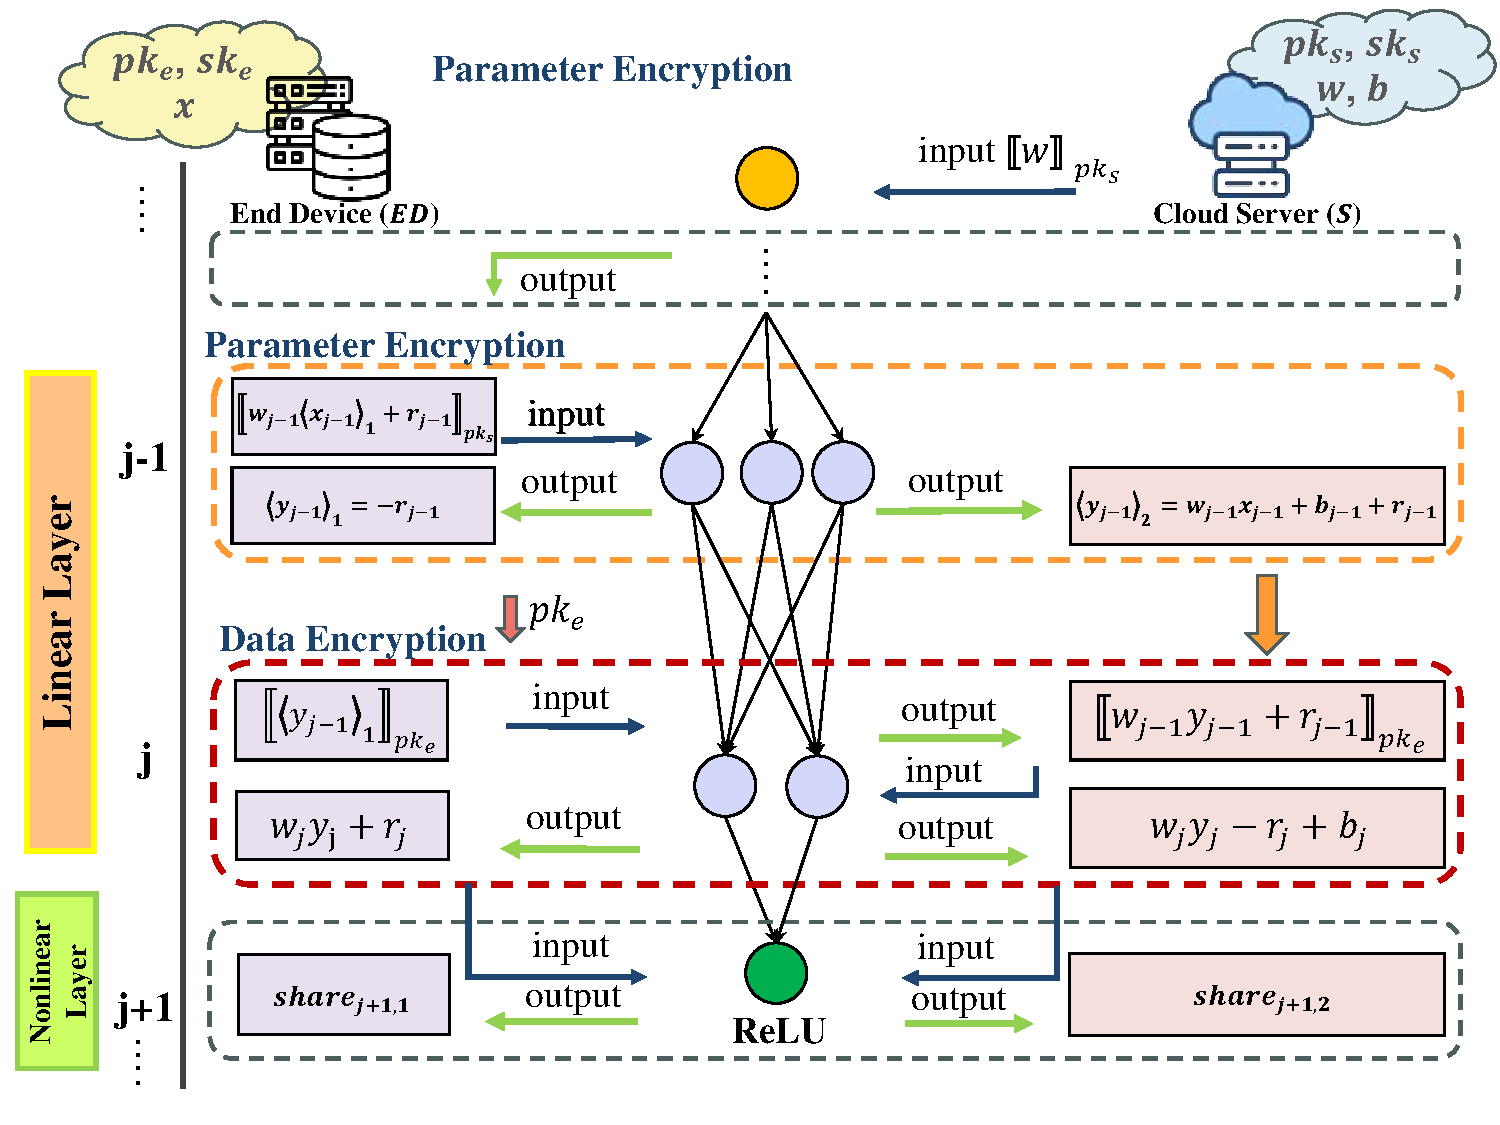
\includegraphics[scale=0.7]{fig3.pdf}
\caption{MIND Overview.} \label{fig:MIND Overview}
\end{figure*}

% \begin{figure}[ht]
% 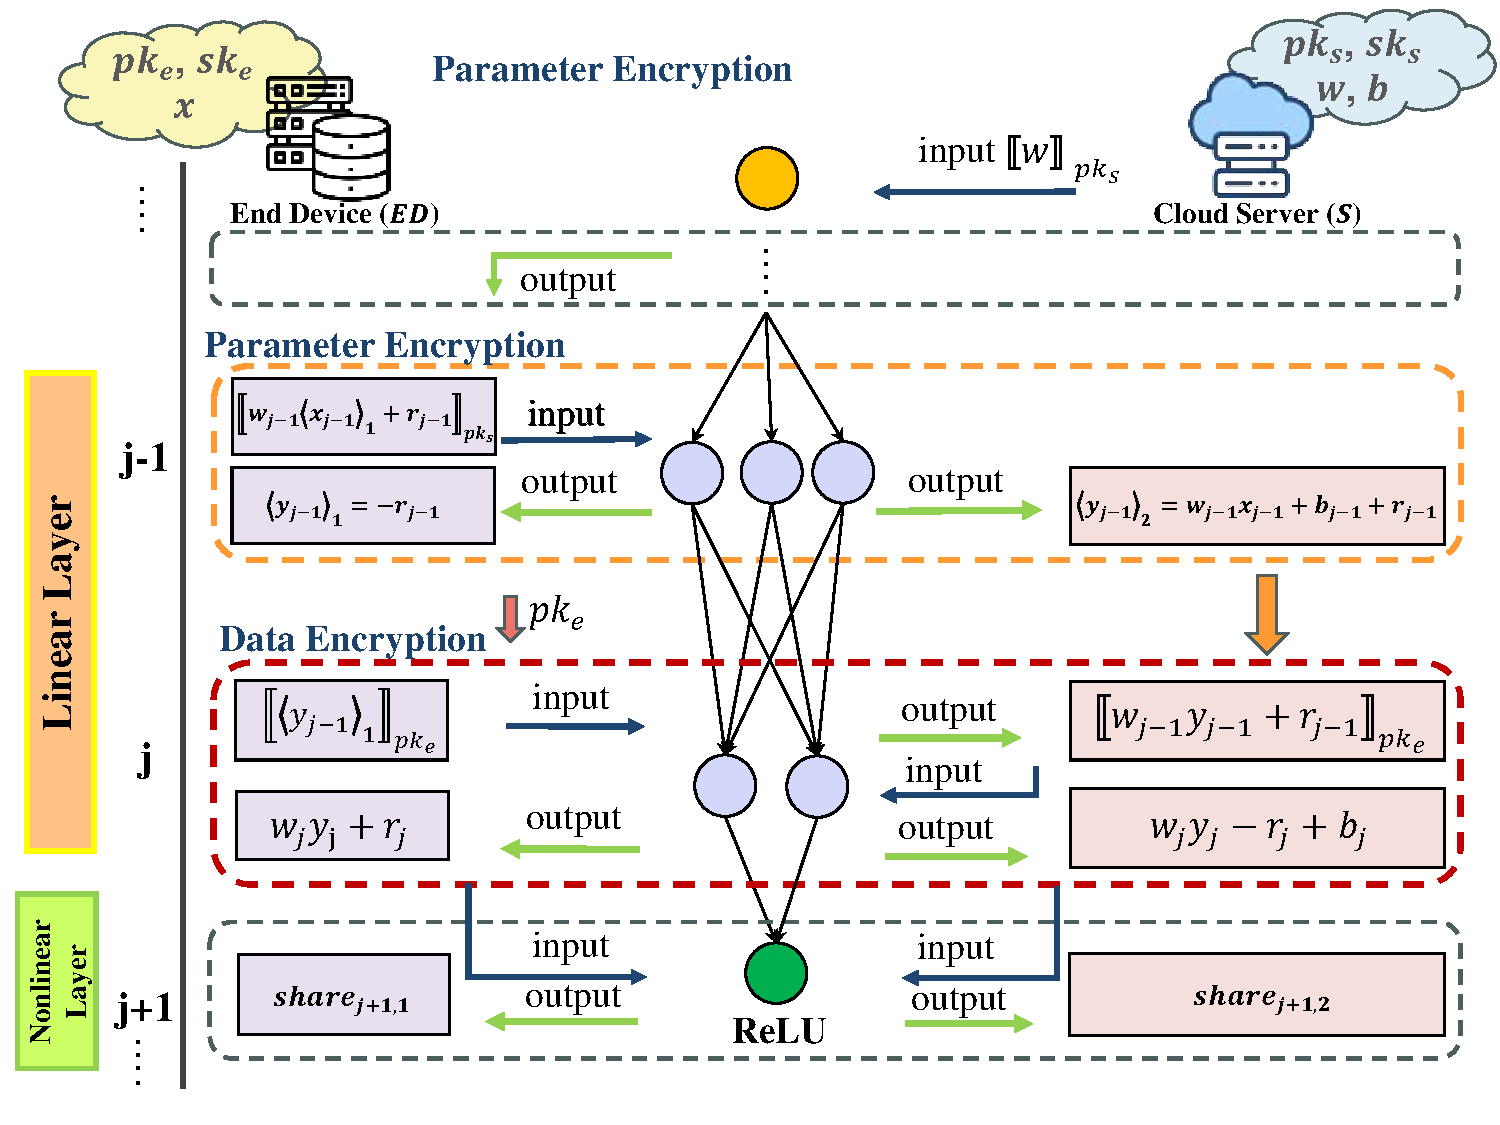
\includegraphics[width=1\linewidth]{fig3.pdf}
% \caption{System model.} \label{fig:MIND Overview}
% \end{figure}

In this inference process, we consider $ED$ holds an image $img$ with the size $n\times m$, and a main computational cloud server $S$ storing the model $M$. The model $M$ is consisted of a sequence of sub-models: $M=M_1 || M_2 || \dots || M_l$, where each model $M_j$ is characterized by specific weights $w_{j}$ and biases $b_{j}$ for $j \in \{1, 2, \dots, l\}$. Formally, $M$ can be represented as a collection of layer-specific parameters $M=\{(w_{1},b_{1}),(w_{2},b_{2}),\dots,(w_{l},b_{l})\}$, where $l$ denotes the number of layers in $M$. This representation encapsulates the complete structure of the neural network model.

The computation at each layer is denoted as $x_j = f_j(x_{j-1})$, where $x_j=\langle x_j \rangle_1 + \langle x_j \rangle_2$. Here, $\langle x_j \rangle_1$ and $\langle x_j \rangle_2$ represent secret shares held by $ED$ and $S$ respectively. The secure computation protocol $f_j$ generates these shares according to the following equation:
\begin{equation}
    \langle x_j \rangle_1+\langle x_j \rangle_2 = f_j(\langle x_{j-1} \rangle_1 + \langle x_{j-1} \rangle_2).
\end{equation}

As described in Algorithm \ref{algo:search}, the process begins with initialization. $ED$ sets the initial secret share as $\langle x_0 \rangle
_1=x$, and $S$ sets $\langle x_0 \rangle
_2=0$. The inference computation proceeds layer by layer. For linear layers, $ED$ and $S$ decide between two encryption protocols (\PEnc~and \DEnc) based on a comparison of the number of bits of parameters in the model ($N_p$) and the number of bits of data in the model ($N_d$). Specifically, when $N_p \leq N_d$, \PEnc~is chosen, where the parameters ($w_j$ and $b_j$) are encrypted and sent for computation. When $N_p > N_d$, \DEnc~is applied, where the input data $\langle x_{j-1} \rangle_1 + \langle x_{j-1} \rangle_2$ is encrypted instead. For non-linear layers, a separate protocol handles their computation securely.

Finally, $S$ sends the resulting secret share $\langle y \rangle_2$ back to $ED$, where $ED$ reconstructs the final inference result $y$ as $y=\langle y \rangle_1 + \langle y \rangle_2$.

\begin{algorithm}[htbp]
	\caption{The Search Procedure}
	\label{algo:search}
	\LinesNumbered
	\KwIn{
	$ED$ holds an image $x$ and batchsize $B$.
	Server $S$ holds the network model $M = M_1 || M_2 || \dots || M_l$.
	The weights and biases of each layer $M_j$ are $w_j$ and $b_j$, respectively.
% 	Define $k$ as the number of model cut layers.
	}
	\KwOut{
	The final inference result $y$
	}
    $ED$ sets $\langle x_0 \rangle_1=x$ and  $S$ sets the $\langle x_0 \rangle_2 = 0$.
    
    % $S$ sends $\llbracket w \rrbracket_{pk_s}$ to $ED$.
	\For{$j=1$ to $l$}{
	    \eIf{The current layer is a linear layer}{
	        \eIf{$ N_{p} \leq N_{d}$}{
	            $(\langle x_{j} \rangle_1$, $\langle x_{j} \rangle_2 ) \leftarrow$ $\PEnc(\langle x_{j - 1}\rangle_1,\langle x_{j-1}\rangle_2,w_j,b_j)$;
	        }{
	             $(\langle x_{j} \rangle_1$, $\langle x_{j} \rangle_2 ) \leftarrow$ $\DEnc(\langle x_{j - 1}\rangle_1,\langle x_{j-1}\rangle_2,w_j,b_j)$;
	        }
	       }{ 
	        Use of non-linear layer protocols{}.
	       }
	   }
	    
    $ED$ defines $\langle y \rangle_1=\langle x_l \rangle_1$ and  $S$ defines the $\langle y \rangle_2=\langle x_l \rangle_2$.
    
   $S$ sends $\langle y \rangle_2$ to $ED$.
    
    $ED$ reconstructs the final inference result by computing $y = \langle y \rangle_1 + \langle y \rangle_2$.
\end{algorithm}

% The core of the process involves layer-wise computation. For each layer $j$ from 1 to $l$, the computation method varies based on the layer's position. For the initial layers $(j \leq k)$, $ED$ uses homomorphic encryption proposed in \PEnc~to perform inference. After applying the \PEnc~method, $ED$ holds the partial encrypted share $\langle x_j \rangle_1$ of the activation value at layer $j$, and $S$ holds the corresponding partial encrypted share $\langle x_j \rangle_2$. As the process moves to later layers $(j > k)$, the method switches to \DEnc, with $S$ continuing the inference using the encrypted data received from $ED$. This switch to \DEnc~in later layers is due to the fact that as the number of neural network layers increases, the computational cost of parameter encryption becomes greater than that of data encryption. Therefore, using the \DEnc~method in later layers can improve computational efficiency.

% After processing all layers, the computation reaches its final stage. At this point, $ED$ holds $\langle y \rangle_1=\langle x_n\rangle_1$ and $S$ holds $\langle y \rangle_2=\langle x_n\rangle_2$. To complete the inference, $S$ sends $\langle y \rangle_2$ to $ED$. $ED$ then reconstructs the final inference result by computing $y=\langle y \rangle_1+\langle y \rangle_2$, effectively combining the shares to produce the output.

% Upon receiving the encrypted parameters, $ED$ uses homomorphic encryption to perform inference on the initial layers. $ED$ then encrypts the resulting intermediate results and sends them to $S$. Subsequently, $S$ continues the inference on the remaining layers using the encrypted data from $ED$. This process ensures that both the sensitive parameters and image data are protected through encryption before further processing or transmission. 

% The computation at each layer is denoted as $x_j = f_j(x_{j-1})$, where $j$ denotes the current network layer and $x_j=\langle x_j \rangle_1 + \langle x_j \rangle_2$. All intermediate outputs of each layer are secretly shared between $ED$ and $S$, except for the final output $y$. At the beginning, we keep the secret sharing form for all layers $f_j$. Here, $f_j$ represents a secure computation protocol running on secret sharing. The protocol obtains the secret share $\langle x_{j-1} \rangle_i$ of the previous layer's output from both parties and generates the secret share $\langle x_j \rangle_i$ of the current layer. This can be expressed as:
% \begin{equation}
%     \langle x_j \rangle_1+\langle x_j \rangle_2 = f_j(\langle x_{j-1} \rangle_1 + \langle x_{j-1} \rangle_2).
% \end{equation}

% % as shown in Fig. \ref{fig:ED_Models} and \ref{fig:Serve_Models}, $ED$ separates the original image feature vector $x$ using an additive secret sharing scheme. 
% Specifically, as described in Algorithm \ref{algo:search}, the initial input is $x_0=x$ split between  $ED$ and $S$, with $ED$ setting $\langle x_0\rangle_1=x$ and $S$ setting the $\langle x_0\rangle_2=0$. 

% For each layer $j$ from 1 to $n$, if $j \leq k$ (where $k$ is the number of layers processed by the $ED$), the $ED$ and $S$ use the \PEnc~method to compute the encrypted shares $\langle x_j \rangle_1$ and $\langle x_j \rangle_2$. Otherwise, we use \DEnc~method.
%  After all layers are processed, $ED$ holds $\langle y \rangle_1=\langle x_n\rangle_1$ and $S$ holds $\langle y \rangle_2=\langle x_n\rangle_2$. Finally, $S$ then sends $\langle y \rangle_2$ to $ED$, which then reconstructs the final inference result by computing $y=\langle y \rangle_1+\langle y \rangle_2$.

In summary, this algorithm ensures that the computational process is carried out securely and efficiently, with the server only having access to a share of the data. By employing secret sharing and encryption techniques, the privacy of the input image is preserved throughout the inference procedure, thereby providing a robust solution for end-cloud collaborative privacy-preserving inference computations.
%In forward propagation, $ED$ draws a batch of input data $\langle x_0\rangle_1$ to feed into the model $M_1$.  


% The overall model $m$ is composed of multiple sub-models $m=\{m_1,m_2,\dots,m_n\}$. Each sub-model $m_i$ consists of several layers, and for each layer $j$ in the sub-model $m_i$, there are associated weights $w_{ij}$ and biases $b_{ij}$. 
% Formally, each sub-model $m_i$ can be represented as a collection of layer-specific parameters $m_i=\{(w_{i1},b_{i1}),(w_{i2},b_{i2}),\dots,(w_{ik},b_{ik})\}$, where $k_i$ denotes the number of layers in $m_i$. Therefore, the overall model m can be expressed as $m =\{(w_{i1}, b_{i1}), (w_{i2}, b_{i2}), \dots,$ $(w_{ik_i}, b_{ik_i}) | i=1,2,\dots,n\}$, with each $m_i$ containing its corresponding set of weights and biases for each layer.

\section{Experimental Evaluations}

In this section, we first compare the effectiveness of MIND and previous work Pencil\cite{liu2024pencilprivateextensiblecollaborative} in terms of effectiveness, including accuracy, precision, recall and F1 score.
The encryption method proposed by MIND encrypts user inputs or server parameters based on the characteristics of each layer, whereas Pencil only encrypt user inputs.
Subsequently, we compare the efficiency and communication complexity of MIND with that of Pencil.







\subsection{Setting}
\subsubsection{Environment} Our experiments are conducted on two servers, each equipped with an AMD EPYC 7402 CPU and 128 GB of RAM.






\subsubsection{Datasets} 
We use the MNIST dataset\cite{xiao2017fashion}a widely recognized benchmark in machine learning and computer vision research. MNIST consists of 70,000 grayscale images of handwritten digits, including 60,000 training samples and 10,000 test samples. Each image is represented as a 28$\times$28 pixel matrix, where each pixel indicates the intensity of grayscale values ranging from 0 to 255. 
% The CIFAR-10 dataset is a classic image classification dataset consisting of 60000 32 × 32 color images from 10 categories, with 50000 for training and 10000 for testing. These categories include airplanes, cars, birds, cats, deer, dogs, frogs, horses, boats, and trucks. 
% These datasets are widely used for developing and evaluating image classification models due to their simplicity and versatility. 
It serves as standards for testing various preprocessing, feature extraction, and classification techniques, providing a consistent basis for evaluating model performance.
% We employ the widely used MNIST\cite{xiao2017fashion} to train and evaluate our models. To ensure the data is suitable for model input, the following preprocessing steps are applied. The MNIST dataset consists of 60,000 training images and 10,000 test images, each a 28$\times$28 pixel grayscale image of handwritten digits. We normalize the pixel values to the [0, 1] range and implemente data augmentation techniques such as random rotations and translations during training. We standardize these images so that pixel values for each channel have zero mean and unit variance. We train each neural network on the training dataset for 10 epochs. To further improve the model's generalization ability, we apply data augmentation techniques, including random cropping, horizontal flipping, and color jittering.
% \subsubsection{Parameters} 
% The learning rate $\eta$ is set to 0.01 to accelerate model convergence while maintaining stability. For the MNIST dataset, a batch size $B$ of 32 is used. The momentum $\gamma$ is configured at 0.8 to effectively smooth the update process and reduce gradient oscillations during training. Additionally, the gradient bound estimation $C$ is set to 8 to limit the gradient's maximum value, preventing gradient explosion.

\subsubsection{Models}
We chose four commonly used neural networks in privacy-preserving machine learning \cite{liu2024pencilprivateextensiblecollaborative} for subsequent experiments.


\begin{itemize}
    \item Network-A.
    Network-A is a fully connected deep neural network (DNN) designed for MNIST classification. It starts with a Flatten layer converting 1×28×28 input into a vector of size 784. The first Linear layer maps size 784 to 128 with ReLU, followed by another Linear layer mapping size 128 to 128 with ReLU. The final Linear layer maps size 128 to 10, representing class probabilities.
    \item Network-B.
    Network-B is a 3-layer CNN for MNIST classification. It begins with a Conv2d layer (input: 1×28×28, kernel: 5×5, stride: 2, padding: 2) producing 5 output channels (5×14×14), followed by ReLU. A Flatten layer converts the feature map into a vector of size 980. A Linear layer maps this to size 100, followed by ReLU, and another Linear layer maps it to size 10 for classification probabilities.
    \item Network-C.
    Network-C is a 5-layer CNN for MNIST classification. It starts with a Conv2d layer (kernel size 5×5, 16 output channels) reducing the input size from 1×28×28 to 16×24×24, followed by ReLU and AvgPool2d (stride 2), resulting in 16×12×12. A second Conv2d layer (16 output channels, kernel (5×5) reduces the size to 16×8×8, followed by ReLU and AvgPool2d, yielding 16×4×4. The feature map is flattened into a vector of size 256, passed through a Linear layer (256 to 100, with ReLU) and another Linear layer (100 to 10) for classification.
    \item Network-D.
    Network-D is a 3-layer Deep Neural Network (DNN) designed for MNIST classification. It starts with a Flatten layer that converts the input 1×28×28 into a vector of size 784. The first Linear layer maps this vector to size 512, followed by a ReLU activation. The second Linear layer maps the vector of size 512 to another vector of size 512, also followed by ReLU. The final Linear layer maps the vector of size 512 to size 10, representing class probabilities.
    % \item AlexNet.
    % AlexNet is a classic convolutional neural network structure consisting of 8 layers, where the first 5 layers are convolutional layers used to extract image features, and the last 3 layers are fully connected layers used for classification tasks, ultimately outputting class probabilities through Softmax.
    % \item ResNet50.
    % ResNet-50 consists of an initial convolutional layer and a max pooling layer, followed by four residual stages, each stage containing several residual modules, each module having three convolutional layers, for a total of fifty layers. Finally, the classification results are output through a global average pooling layer and a fully connected layer.
    
\end{itemize}











\subsection{Effectiveness}
In this subsection, we compare the effectiveness of secure inference across different networks on the MNIST dataset with MIND and Pencil \cite{liu2024pencilprivateextensiblecollaborative}.
Specifically, the evaluation focuses on comparing the accuracy, precision, recall, and F1 score between MIND and Pencil.
MIND starts by proposing a layer-wise adaptive encryption method, which encrypts the data and parameters with relatively smaller sizes at each layer, while Pencil only encrypts the data.




% In this subsection, we evaluate the effectiveness of the scheme. The MIND scheme we propose employs a hierarchical encryption method, while Pencil \cite{liu2024pencilprivateextensiblecollaborative} is a non layered encryption scheme. 


% We evaluate the performance using models with different architectures on the MNIST dataset, specifically ABY3\cite{10.1145/3243734.3243760}, Sphinx\cite{Tian2022SphinxEP}, Chameleon\cite{10.1145/3196494.3196522} and Quotient 2$\times$512\cite{10.1145/3319535.3339819}. The evaluation focuses on comparing the accuracy, precision, recall, and F1 score between the hierarchical and non-hierarchical encryption schemes using these MNIST models.




% Based on the results presented in Figure \ref{fig:ACC}, we observe no significant difference in recognition accuracy between the layered and non-layered encryption scheme. This demonstrates that our proposed MIND scheme effectively maintains model performance while implementing enhanced privacy protection measures.




% The data presented in Table \ref{tab:performance_comparison_scheme} indicates that all tested models perform consistently in both the Pencil and MIND schemes. In the MNIST dataset, protocols like ABY3, Chameleon, Sphinx, and Quotient show nearly identical precision, recall, and F1 scores in both environments. 




Table \ref{tab:performance_comparison_scheme} shows that when using Network-A for privacy-preserving secure inference on the MNIST dataset, MIND achieves an accuracy, precision, recall, and F1 score of 0.978, 0.978, 0.978, and 0.978, respectively.
In contrast, Pencil achieves an accuracy, precision, recall, and F1 score of 0.978, 0.978, 0.978, and 0.978, respectively. The performance of the remaining networks is similar.




The results indicate that when performing secure inference on the MNIST dataset using different networks, MIND exhibits nearly identical precision, recall, and F1 scores compared to previous secure inference work \cite{liu2024pencilprivateextensiblecollaborative}.
It is worth noting that MIND does not significantly affect model effectiveness, especially in simpler tasks. 
This suggests that MIND is effective in achieving privacy preserving secure inference while maintaining model accuracy.











\begin{table}[ht]
\centering
\caption{Performance comparison between Pencil and MIND models for different tasks.}
\begin{tabular}{ l|l|l | c c c c } 
\hline
\multirow{2}{*}{Dataset} & \multirow{2}{*}{Network} & \multirow{2}{*}{Scheme} & \multicolumn{4}{c}{Metric} \\ 
\cline{4-7}
                      &                        &                        & \textbf{Acc.} & \textbf{Rec.} & \textbf{F1} & \textbf{Prec.} \\ 
\hline
\multirow{8}{*}{MNIST}   & \multirow{3}{*}{Network-A}  
                         & Baseline & 0.978 & 0.978 & 0.978 & 0.978 \\ 
                         &           & Pencil & 0.978 & 0.978 & 0.978 & 0.978 \\ 
                         &            & MIND    & 0.978 & 0.978 & 0.978 & 0.978 \\ 
\cline{2-7}
                      & \multirow{3}{*}{Network-B}
                      & Baseline & 0.985 & 0.985 & 0.985 & 0.985 \\
                      &           & Pencil & 0.985 & 0.985 & 0.985 & 0.985 \\ 
                      &            & MIND    & 0.985 & 0.985 & 0.985 & 0.985 \\ 
\cline{2-7}
                      & \multirow{3}{*}{Network-C}    
                      & Baseline & 0.9910 & 0.9911 & 0.9910 & 0.9910 \\
                      &          & Pencil & 0.991 & 0.990 & 0.991 & 0.991 \\ 
                      &            & MIND    & 0.991 & 0.990 & 0.991 & 0.991 \\ 
\cline{2-7}
                      & \multirow{3}{*}{Network-D}
                      & Baseline & 0.9812 & 0.9814 & 0.9810 & 0.9812 \\
                      &         & Pencil & 0.981 & 0.981 & 0.981 & 0.981 \\ 
                      &            & MIND    & 0.981 & 0.981 & 0.981 & 0.981 \\ 
\hline
% \multirow{4}{*}{CIFAR-10} & \multirow{2}{*}{AlexNet}    & Pencil  &  0.867  & 0.866  & 0.867 & 0.867  \\ 
%                       &            & MIND    &  0.867  & 0.866  & 0.867 & 0.867  \\ 
% \cline{2-7}
%                       & \multirow{2}{*}{ResNet50}    & Pencil  & 0.819 & 0.767 & 0.785 & 0.805 \\ 
%                       &            & MIND    & 0.819 & 0.767 & 0.785 & 0.805\\ 
% \cline{2-7}
                    %   & \centering DenseNet121 & Native  & 0.649 & 0.597 &0.622  \\ 
                    %   &            & MIND    & 0.649 & 0.597 &0.622 \\ 
                    
\hline
\end{tabular}
\vspace{-2pt}   % 调整表格与Note的距离
\begin{flushleft}
\begin{adjustwidth}{2pt}{2pt}  % 这里调整Note与左右边界的距离
\textbf{Note.}
$\text{Accuracy} = \frac{\text{TP} + \text{TN}}{\text{TP} + \text{TN} + \text{FP} + \text{FN}}$,
$\text{Precision} = \frac{\text{TP}}{\text{TP} + \text{FP}}$,
$\text{Recall} = \frac{\text{TP}}{\text{TP} + \text{FN}}$,
$\text{F1 Score} = 2 \times \frac{\text{Precision} \times \text{Recall}}{\text{Precision} + \text{Recall}}$ 
(TP: True Positive, TN: True Negative, FP: False Positive, FN: False Negative).
\end{adjustwidth}
\end{flushleft}
\label{tab:performance_comparison_scheme}
\end{table}




% \begin{table*}[ht]
% \centering
% \caption{Feasibility Evaluation}
% \label{tab:effectiveness}
% \begin{tabular}{lcccccc}
% \toprule[1pt]
% Model & Schemes & Precision & Recall & F1 Score  \\
% \midrule[1pt]
% \multirow{2}{*}{MNIST ABY3} & Naive & 0.978 & 0.978 & 0.978  \\
%                             & MIND & 0.978 & 0.978 & 0.978  \\ \cline{1-6}
% \multirow{2}{*}{MNIST Sphinx} & Naive & 0.991 & 0.990 & 0.991  \\
%                             & MIND & 0.991 & 0.990 & 0.991  \\ \cline{1-6}
% \multirow{2}{*}{MNIST Quotient 3$\times$128} & Naive & 0.978 & 0.978 & 0.978  \\
%                             & MIND & 0.978 & 0.978 & 0.978  \\ \cline{1-6}
% \multirow{2}{*}{MNIST Quotient 2$\times$512} & Naive & 0.980 & 0.980 & 0.980  \\
%                             & MIND & 0.980 & 0.980 & 0.980  \\ \cline{1-6}
% \bottomrule[1pt]
% \end{tabular}
% \vspace{-6pt}
% \begin{flushleft}
% \begin{adjustwidth}{90pt}{70pt}  % 这里调整Note与左右边界的距离
% \textbf{Note.}
% $\text{Accuracy} = \frac{\text{TP} + \text{TN}}{\text{TP} + \text{TN} + \text{FP} + \text{FP}}$,
% $\text{Precision} = \frac{\text{TP}}{\text{TP} + \text{FP}}$,
% $\text{Recall} = \frac{\text{TP}}{\text{TP} + \text{FP}}$,
% $\text{F1 Score} = 2 \times \frac{\text{Precision} \times \text{Recall}}{\text{Precision} + \text{Recall}}$ 
% (TP: True Positive, TN: True Negative, FP: False Positive, FN: False Negative).
% \end{adjustwidth}
% \end{flushleft}
% \end{table*}

\subsection{Efficiency}

\begin{figure}[ht]
    \centering
    \subfigure[Network-A]{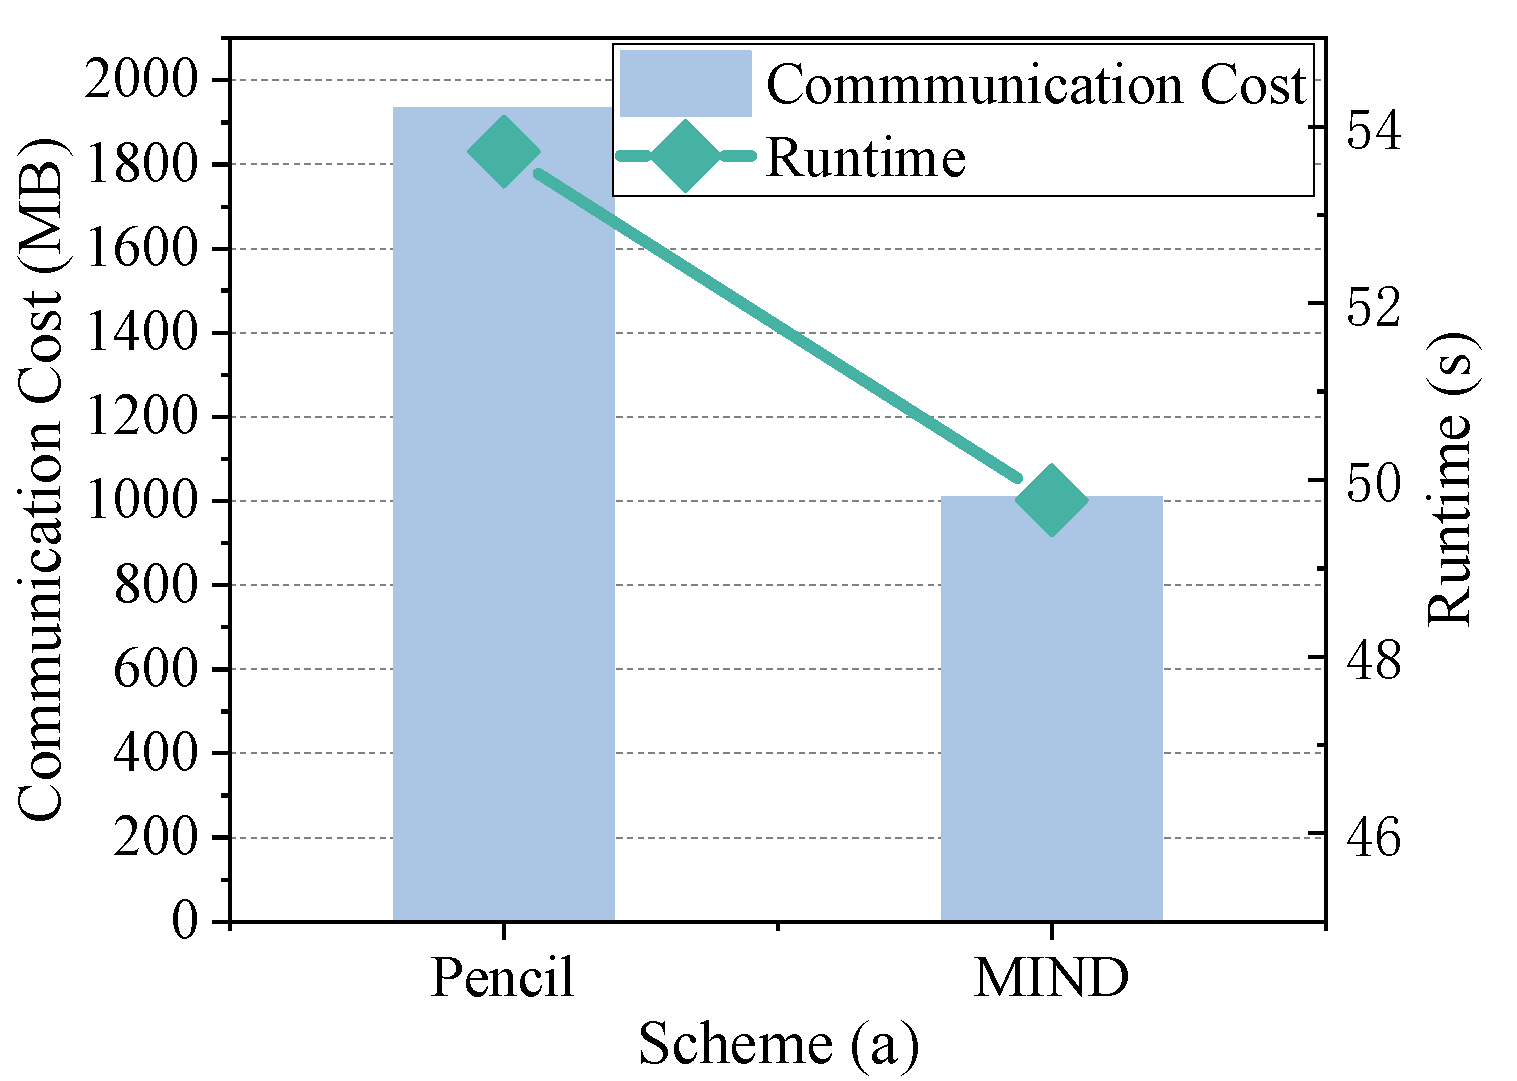
\includegraphics[width=.45\columnwidth]{exp/ABY3.pdf}\label{subfig:ABY3}} \hspace{5pt}
    % \subfigure[MNIST Quotient 3$\times$128]{\includegraphics[width=.45\columnwidth]{exp/Quotient_3.pdf}\label{subfig:Quotient_3x128}} \hspace{5pt}
    \subfigure[Network-B]{\includegraphics[width=.45\columnwidth]{exp/Chameleon.pdf}\label{subfig:Chameleon}} \hspace{5pt}\\
    \subfigure[Network-C]{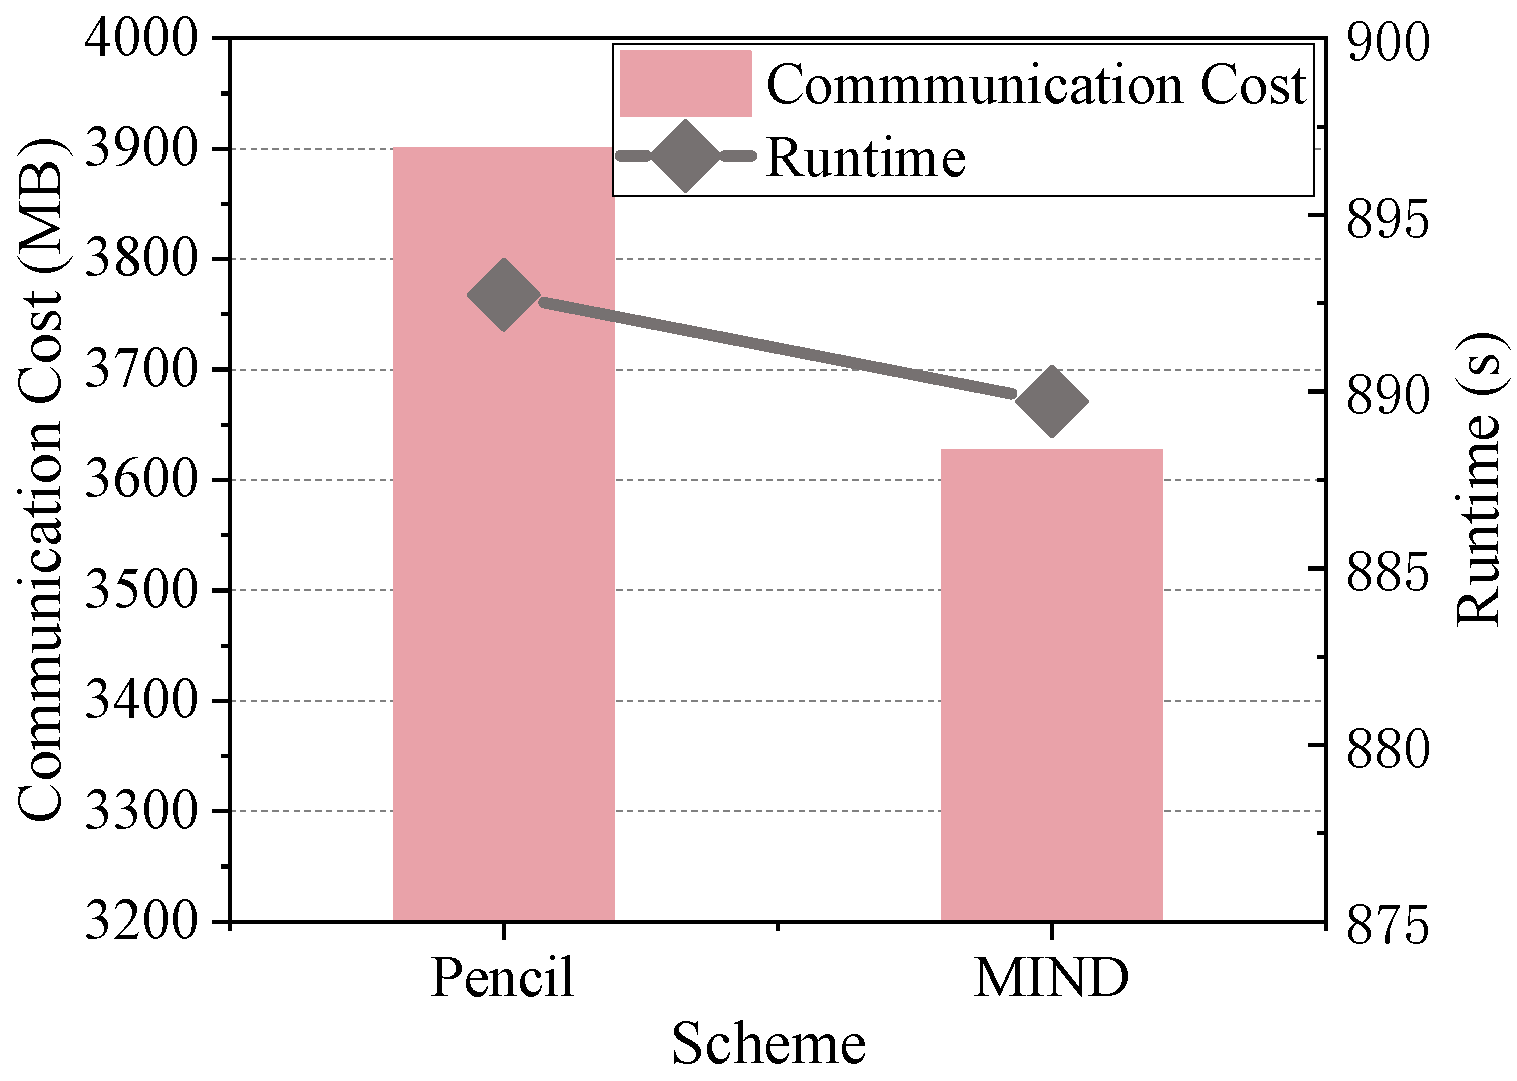
\includegraphics[width=.45\columnwidth]{exp/Sphinx.pdf}\label{subfig:Sphinx}} 
    \subfigure[Network-D %2$\times$512%
     ]{\includegraphics[width=.45\columnwidth]{exp/Quotient_2.pdf}\label{subfig:Quotient_2x512}}
    
    % \subfigure[AlexNet]{\includegraphics[width=.467\columnwidth]{exp/AlexNet.pdf}\label{subfig:AlexNet}} \hspace{2pt}
    % \subfigure[ResNet50]{\includegraphics[width=.47\columnwidth]{exp/ResNet.pdf}\label{subfig:ResNet}} 
    % \caption{Efficiency evaluation.}
    % \label{fig:efficiency}
\end{figure}
% \begin{figure}[ht]
% \centering
% 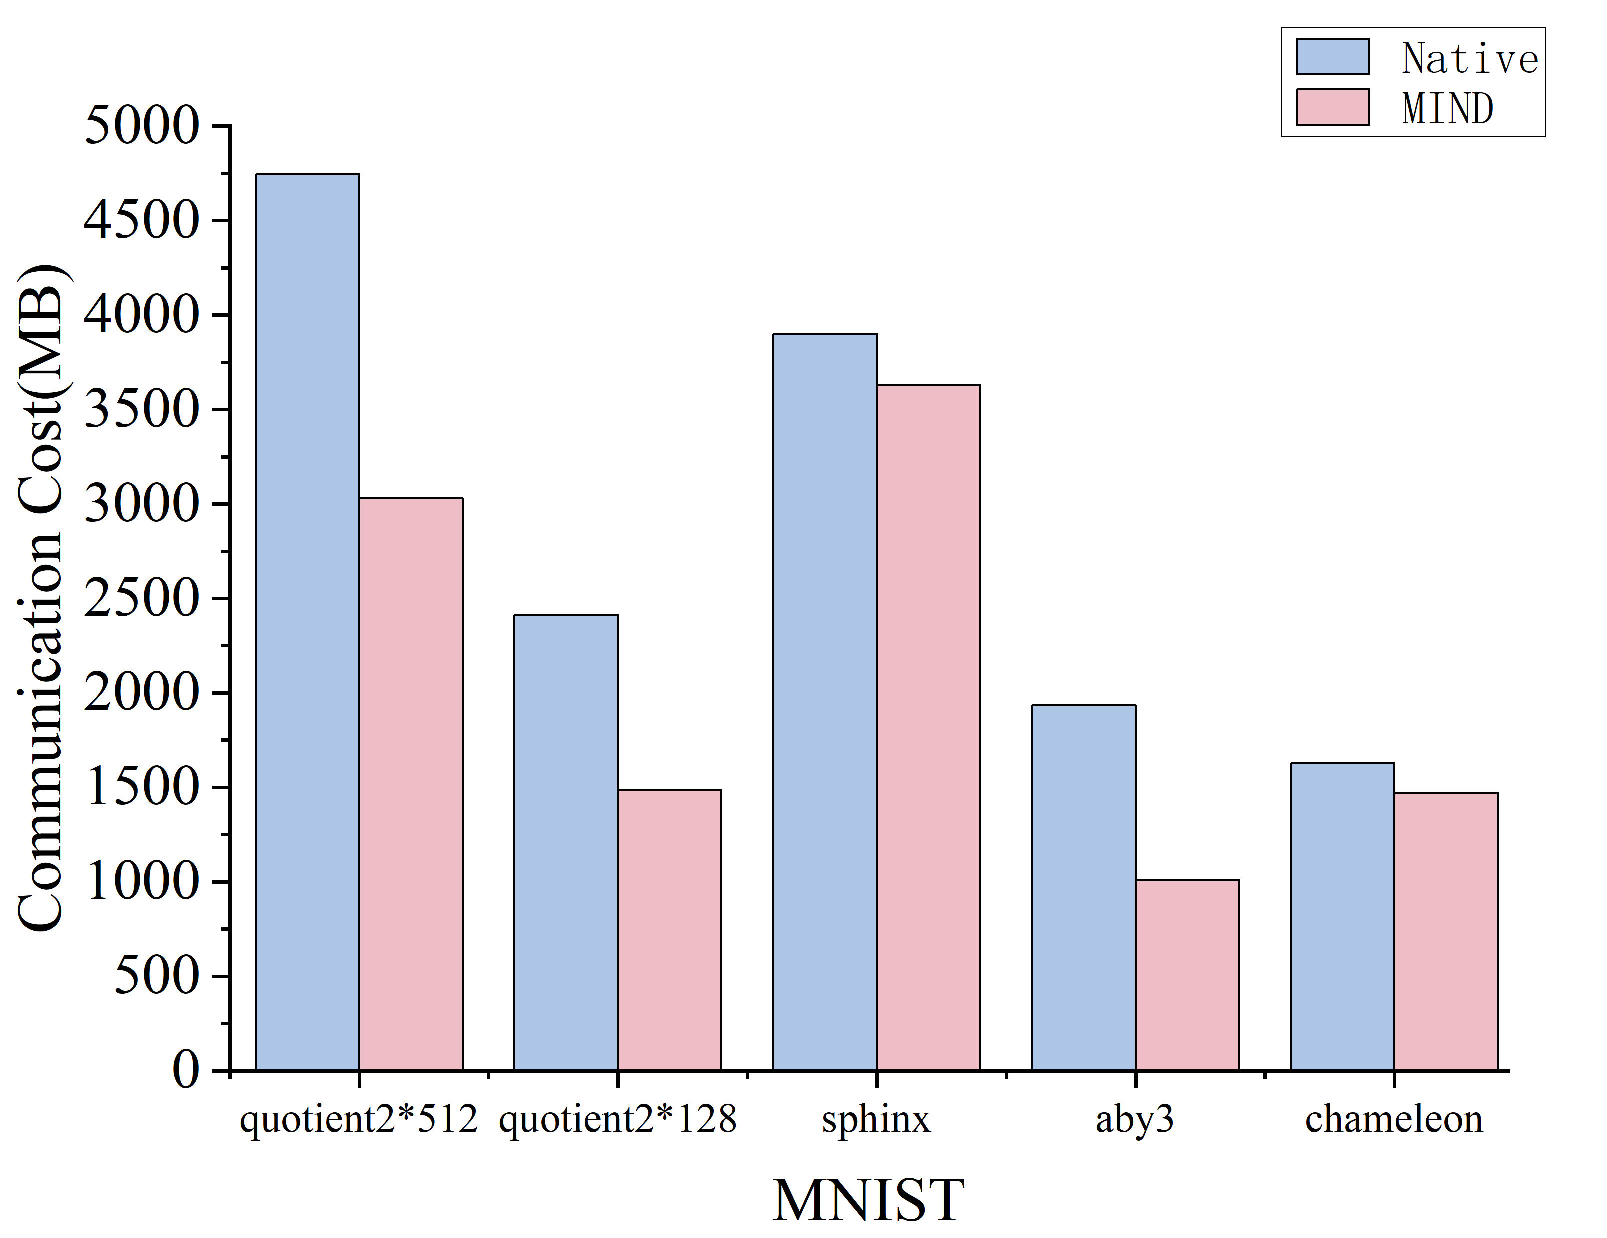
\includegraphics[width=1\linewidth]{Communication_cost.pdf}
% \caption{Communication cost} \label{fig:cost}
% \end{figure}

% To demonstrate MIND's efficiency, in this subsection, we evaluate and compare the computational overhead of Pencil and MIND across different models. Results are averaged across multiple experiments to ensure reliability.
% In the experiment, we use two publicly available datasets, MNIST and CIFAR-10, and apply various models to each dataset. Pretrained models, such as AlexNet and ResNet50, are utilized as feature extractors. As shown in Figure \ref{fig:ACC}, across different models, the accuracy remains almost unchanged when using the MIND method (represented by the pink bars) compared to the native method (represented by the blue bars). This indicates that the impact of the MIND method on model accuracy is almost negligible.




Subsequently, we further compare MIND and Pencil in terms of efficiency and their corresponding communication overhead on the MNIST test set.
% The results are averaged over multiple experiments to ensure reliability.
Specifically, Pencil \cite{liu2024pencilprivateextensiblecollaborative} considers transferring the complex homomorphic operations from the online phase to the offline phase to improve efficiency, and MIND is also applicable to these optimizations.
For fairness, neither MIND nor Pencil adopts the above-mentioned optimization schemes in the experiments.









 



Figure \ref{subfig:ABY3}, \ref{subfig:Sphinx}, \ref{subfig:Chameleon}, and \ref{subfig:Quotient_2x512} show that for the MNIST dataset, MIND consistently requires less transmission and runtime across all four networks compared to Pencil.
% As shown in Figure \ref{subfig:ABY3}, ABY3 is the most efficient in reducing communication cost when applied to the ABY3 model and the most efficient in reducing runtime when applied to the Quotient 2$\times$512 model. Our experiments reveal that while the Pencil encryption scheme requires a communication cost of 1,933 MB, MIND only requires 1,008 MB, resulting in a significant reduction of approximately 49.42\% in communication cost. Additionally, MIND reduces the runtime by approximately 10.34\% compared to the Pencil scheme.
As shown in Figure \ref{subfig:ABY3}, When using network-A, the communication overhead of MIND is 1008MB, and the runtime is 49.8 seconds. Compared with Pencil, the communication overhead is reduced by 925MB, and the efficiency is improved by 7.8\%. When using other networks, MIND reduces communication overhead by 7.5\% to 62.3\% and improves efficiency by 0.3\% to 10.3\% compared to Pencil.

Experiments demonstrate that MIND outperforms Pencil in various network efficiency aspects in the MNIST dataset and CIFA-10 dataset. These results consistently highlight MIND's ability to optimize both communication cost and runtime across various neural network architectures, showcasing its potential for improving efficiency in privacy-preserving machine learning applications.


\section{Conclusion}
In this paper, we presented MIND, an end-cloud collaborative privacy-preserving inference framework by fully taking advantage of the computing capability of the end device and the cloud server. In MIND, no data of the end device and the model parameter of the cloud server are leaked to each other. Specifically, the end device and the cloud server jointly perform secure two-party computations at each layer of the model through the homomorphic cryptosystem, additive secret sharing, or both. MIND shows better performance in terms of runtime due to our architecture design, and the same result in model inference compared to existing work.
For future work, we will explore a pre-computing mechanism to improve the performance of MIND for model inference.


% \subsection{Equations}
% Number equations consecutively. To make your 
% equations more compact, you may use the solidus (~/~), the exp function, or 
% appropriate exponents. Italicize Roman symbols for quantities and variables, 
% but not Greek symbols. Use a long dash rather than a hyphen for a minus 
% sign. Punctuate equations with commas or periods when they are part of a 
% sentence, as in:
% \begin{equation}
% a+b=\gamma\label{eq}
% \end{equation}

% Be sure that the 
% symbols in your equation have been defined before or immediately following 
% the equation. Use ``\eqref{eq}'', not ``Eq.~\eqref{eq}'' or ``equation \eqref{eq}'', except at 
% the beginning of a sentence: ``Equation \eqref{eq} is . . .''

% \subsection{\LaTeX-Specific Advice}

% Please use ``soft'' (e.g., \verb|\eqref{Eq}|) cross references instead
% of ``hard'' references (e.g., \verb|(1)|). That will make it possible
% to combine sections, add equations, or change the order of figures or
% citations without having to go through the file line by line.

% Please don't use the \verb|{eqnarray}| equation environment. Use
% \verb|{align}| or \verb|{IEEEeqnarray}| instead. The \verb|{eqnarray}|
% environment leaves unsightly spaces around relation symbols.

% Please note that the \verb|{subequations}| environment in {\LaTeX}
% will increment the main equation counter even when there are no
% equation numbers displayed. If you forget that, you might write an
% article in which the equation numbers skip from (17) to (20), causing
% the copy editors to wonder if you've discovered a new method of
% counting.

% {\BibTeX} does not work by magic. It doesn't get the bibliographic
% data from thin air but from .bib files. If you use {\BibTeX} to produce a
% bibliography you must send the .bib files. 

% {\LaTeX} can't read your mind. If you assign the same label to a
% subsubsection and a table, you might find that Table I has been cross
% referenced as Table IV-B3. 

% {\LaTeX} does not have precognitive abilities. If you put a
% \verb|\label| command before the command that updates the counter it's
% supposed to be using, the label will pick up the last counter to be
% cross referenced instead. In particular, a \verb|\label| command
% should not go before the caption of a figure or a table.

% Do not use \verb|\nonumber| inside the \verb|{array}| environment. It
% will not stop equation numbers inside \verb|{array}| (there won't be
% any anyway) and it might stop a wanted equation number in the
% surrounding equation.

% \subsection{Some Common Mistakes}\label{SCM}
% \begin{itemize}
% \item The word ``data'' is plural, not singular.
% \item The subscript for the permeability of vacuum $\mu_{0}$, and other common scientific constants, is zero with subscript formatting, not a lowercase letter ``o''.
% \item In American English, commas, semicolons, periods, question and exclamation marks are located within quotation marks only when a complete thought or name is cited, such as a title or full quotation. When quotation marks are used, instead of a bold or italic typeface, to highlight a word or phrase, punctuation should appear outside of the quotation marks. A parenthetical phrase or statement at the end of a sentence is punctuated outside of the closing parenthesis (like this). (A parenthetical sentence is punctuated within the parentheses.)
% \item A graph within a graph is an ``inset'', not an ``insert''. The word alternatively is preferred to the word ``alternately'' (unless you really mean something that alternates).
% \item Do not use the word ``essentially'' to mean ``approximately'' or ``effectively''.
% \item In your paper title, if the words ``that uses'' can accurately replace the word ``using'', capitalize the ``u''; if not, keep using lower-cased.
% \item Be aware of the different meanings of the homophones ``affect'' and ``effect'', ``complement'' and ``compliment'', ``discreet'' and ``discrete'', ``principal'' and ``principle''.
% \item Do not confuse ``imply'' and ``infer''.
% \item The prefix ``non'' is not a word; it should be joined to the word it modifies, usually without a hyphen.
% \item There is no period after the ``et'' in the Latin abbreviation ``et al.''.
% \item The abbreviation ``i.e.'' means ``that is'', and the abbreviation ``e.g.'' means ``for example''.
% \end{itemize}
% An excellent style manual for science writers is \cite{b7}.

% \subsection{Authors and Affiliations}\label{AAA}
% \textbf{The class file is designed for, but not limited to, six authors.} A 
% minimum of one author is required for all conference articles. Author names 
% should be listed starting from left to right and then moving down to the 
% next line. This is the author sequence that will be used in future citations 
% and by indexing services. Names should not be listed in columns nor group by 
% affiliation. Please keep your affiliations as succinct as possible (for 
% example, do not differentiate among departments of the same organization).

% \subsection{Identify the Headings}\label{ITH}
% Headings, or heads, are organizational devices that guide the reader through 
% your paper. There are two types: component heads and text heads.

% Component heads identify the different components of your paper and are not 
% topically subordinate to each other. Examples include Acknowledgments and 
% References and, for these, the correct style to use is ``Heading 5''. Use 
% ``figure caption'' for your Figure captions, and ``table head'' for your 
% table title. Run-in heads, such as ``Abstract'', will require you to apply a 
% style (in this case, italic) in addition to the style provided by the drop 
% down menu to differentiate the head from the text.

% Text heads organize the topics on a relational, hierarchical basis. For 
% example, the paper title is the primary text head because all subsequent 
% material relates and elaborates on this one topic. If there are two or more 
% sub-topics, the next level head (uppercase Roman numerals) should be used 
% and, conversely, if there are not at least two sub-topics, then no subheads 
% should be introduced.

% \subsection{Figures and Tables}\label{FAT}
% \paragraph{Positioning Figures and Tables} Place figures and tables at the top and 
% bottom of columns. Avoid placing them in the middle of columns. Large 
% figures and tables may span across both columns. Figure captions should be 
% below the figures; table heads should appear above the tables. Insert 
% figures and tables after they are cited in the text. Use the abbreviation 
% ``Fig.~\ref{fig}'', even at the beginning of a sentence.

% \begin{table}[htbp]
% \caption{Table Type Styles}
% \begin{center}
% \begin{tabular}{|c|c|c|c|}
% \hline
% \textbf{Table}&\multicolumn{3}{|c|}{\textbf{Table Column Head}} \\
% \cline{2-4} 
% \textbf{Head} & \textbf{\textit{Table column subhead}}& \textbf{\textit{Subhead}}& \textbf{\textit{Subhead}} \\
% \hline
% copy& More table copy$^{\mathrm{a}}$& &  \\
% \hline
% \multicolumn{4}{l}{$^{\mathrm{a}}$Sample of a Table footnote.}
% \end{tabular}
% \label{tab1}
% \end{center}
% \end{table}

% \begin{figure}[htbp]
% \centerline{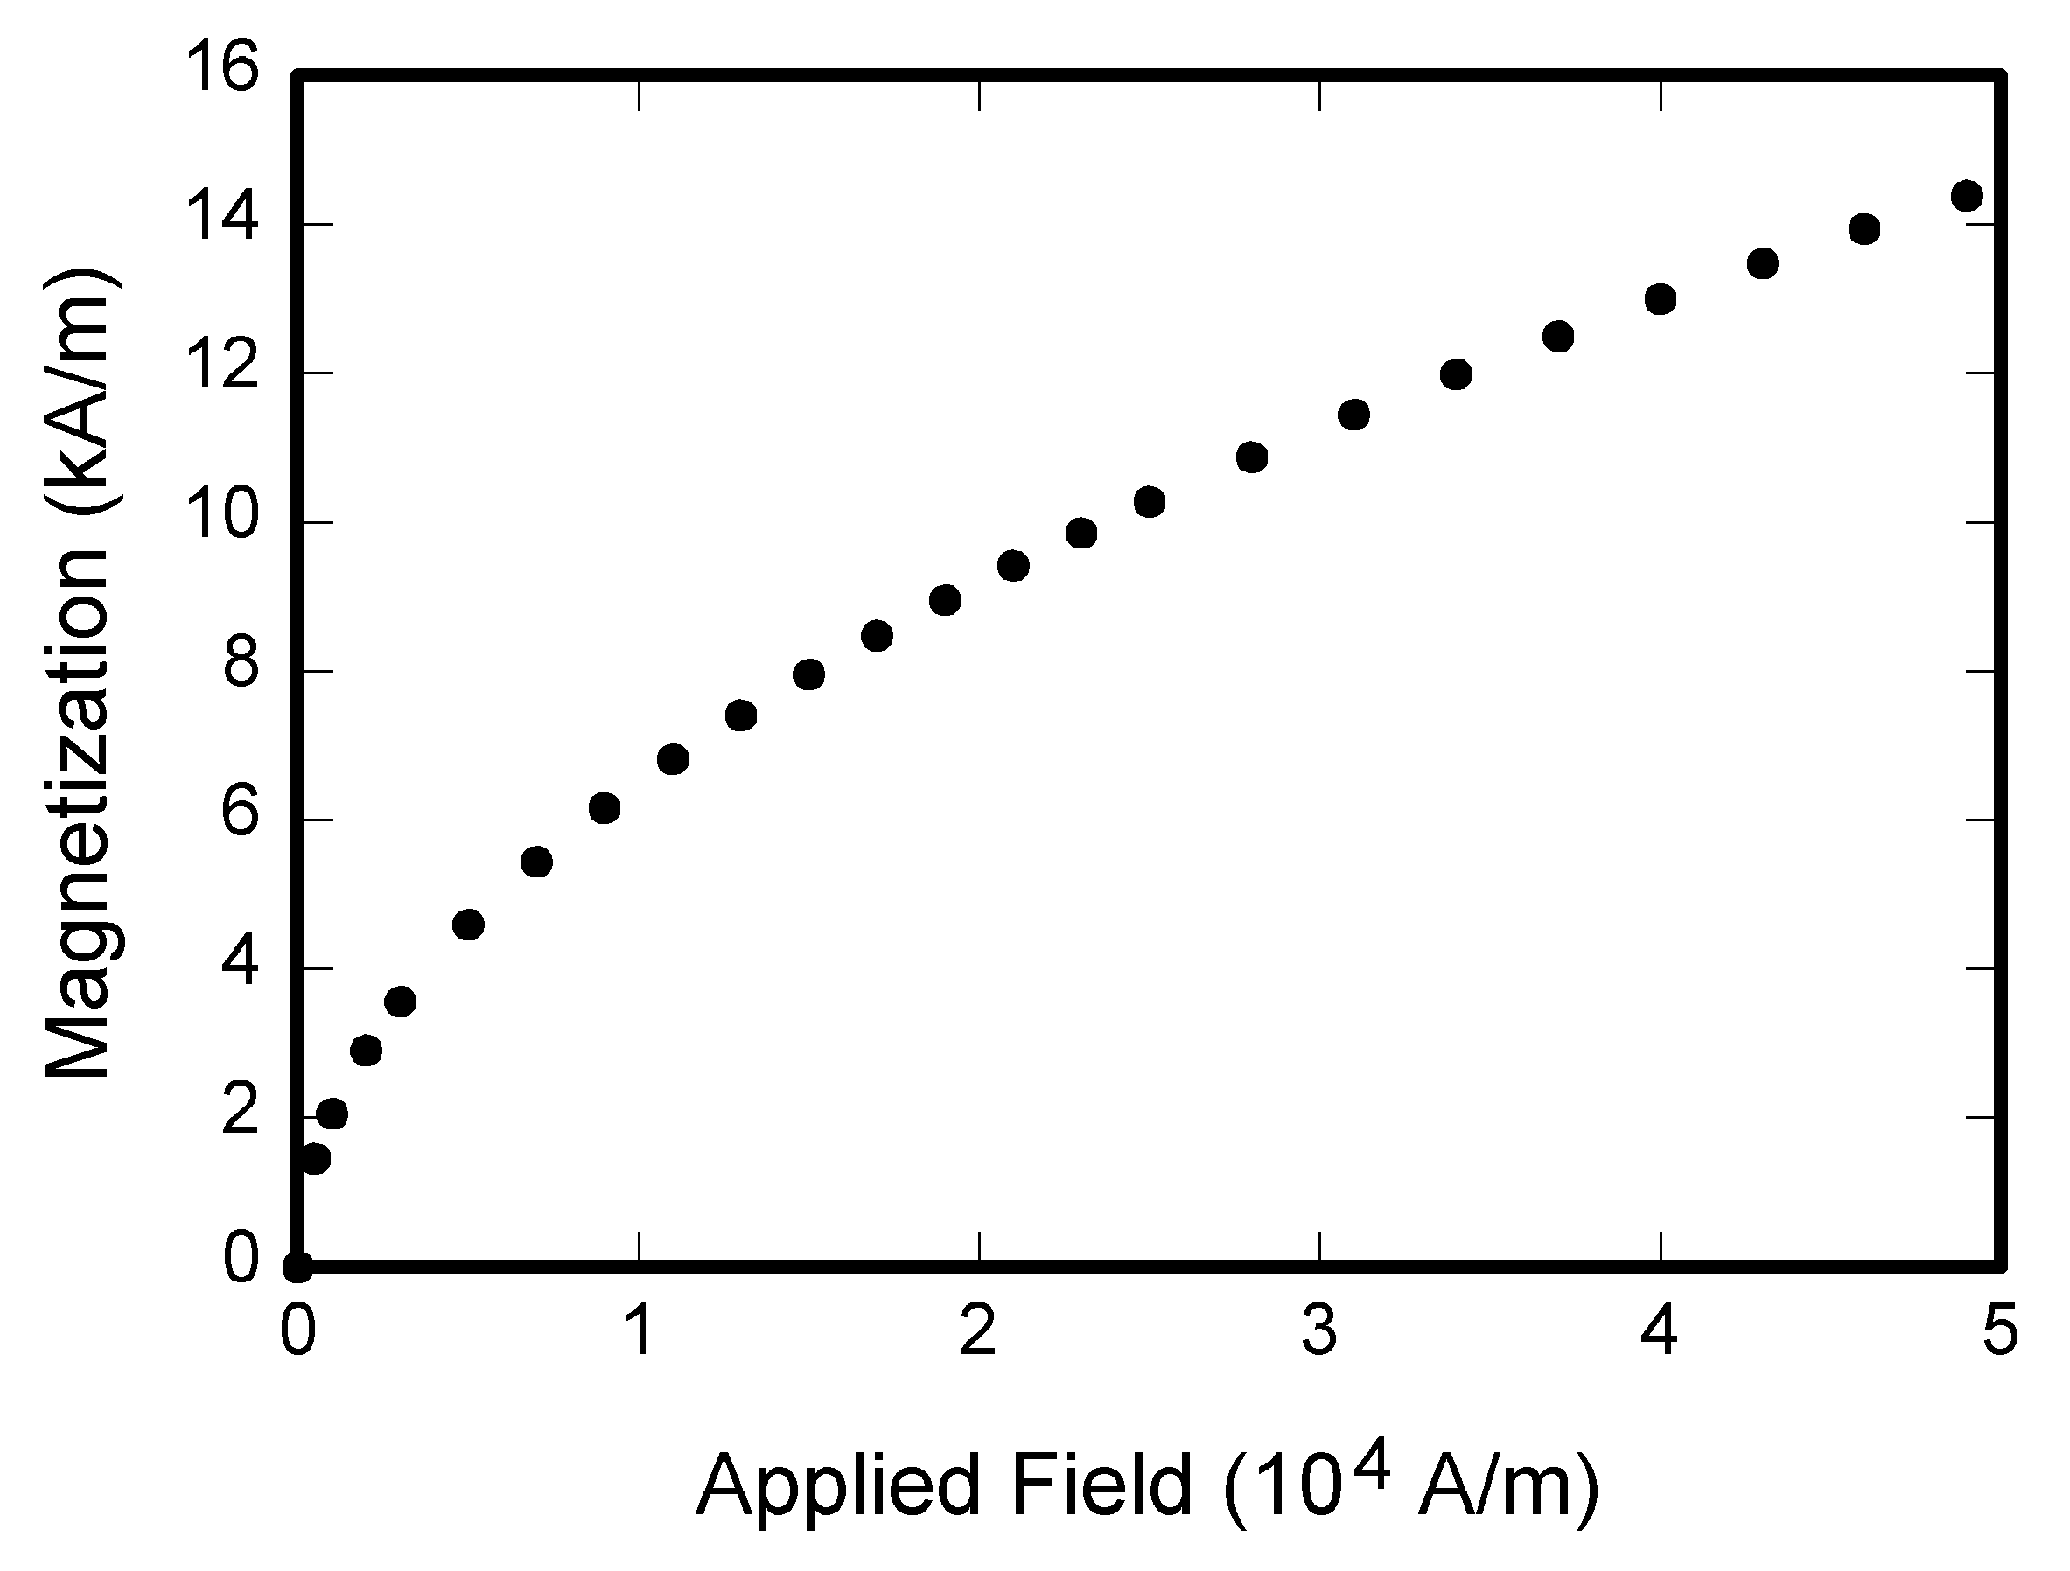
\includegraphics{fig1.png}}
% \caption{Example of a figure caption.}
% \label{fig}
% \end{figure}

% Figure Labels: Use 8 point Times New Roman for Figure labels. Use words 
% rather than symbols or abbreviations when writing Figure axis labels to 
% avoid confusing the reader. As an example, write the quantity 
% ``Magnetization'', or ``Magnetization, M'', not just ``M''. If including 
% units in the label, present them within parentheses. Do not label axes only 
% with units. In the example, write ``Magnetization (A/m)'' or ``Magnetization 
% \{A[m(1)]\}'', not just ``A/m''. Do not label axes with a ratio of 
% quantities and units. For example, write ``Temperature (K)'', not 
% ``Temperature/K''.

% \section*{Acknowledgment}

% The preferred spelling of the word ``acknowledgment'' in America is without 
% an ``e'' after the ``g''. Avoid the stilted expression ``one of us (R. B. 
% G.) thanks $\ldots$''. Instead, try ``R. B. G. thanks$\ldots$''. Put sponsor 
% acknowledgments in the unnumbered footnote on the first page.

% \begin{thebibliography}{00}
% \bibitem{b1} G. Eason, B. Noble, and I. N. Sneddon, ``On certain integrals of Lipschitz-Hankel type involving products of Bessel functions,'' Phil. Trans. Roy. Soc. London, vol. A247, pp. 529--551, April 1955.
% \bibitem{b2} J. Clerk Maxwell, A Treatise on Electricity and Magnetism, 3rd ed., vol. 2. Oxford: Clarendon, 1892, pp.68--73.
% \bibitem{b3} I. S. Jacobs and C. P. Bean, ``Fine particles, thin films and exchange anisotropy,'' in Magnetism, vol. III, G. T. Rado and H. Suhl, Eds. New York: Academic, 1963, pp. 271--350.
% \bibitem{b4} K. Elissa, ``Title of paper if known,'' unpublished.
% \bibitem{b5} R. Nicole, ``Title of paper with only first word capitalized,'' J. Name Stand. Abbrev., in press.
% \bibitem{b6} Y. Yorozu, M. Hirano, K. Oka, and Y. Tagawa, ``Electron spectroscopy studies on magneto-optical media and plastic substrate interface,'' IEEE Transl. J. Magn. Japan, vol. 2, pp. 740--741, August 1987 [Digests 9th Annual Conf. Magnetics Japan, p. 301, 1982].
% \bibitem{b7} M. Young, The Technical Writer's Handbook. Mill Valley, CA: University Science, 1989.
% \bibitem{b8} D. P. Kingma and M. Welling, ``Auto-encoding variational Bayes,'' 2013, arXiv:1312.6114. [Online]. Available: https://arxiv.org/abs/1312.6114
% \bibitem{b9} S. Liu, ``Wi-Fi Energy Detection Testbed (12MTC),'' 2023, gitHub repository. [Online]. Available: https://github.com/liustone99/Wi-Fi-Energy-Detection-Testbed-12MTC
% \bibitem{b10} ``Treatment episode data set: discharges (TEDS-D): concatenated, 2006 to 2009.'' U.S. Department of Health and Human Services, Substance Abuse and Mental Health Services Administration, Office of Applied Studies, August, 2013, DOI:10.3886/ICPSR30122.v2
% \bibitem{b11} K. Eves and J. Valasek, ``Adaptive control for singularly perturbed systems examples,'' Code Ocean, Aug. 2023. [Online]. Available: https://codeocean.com/capsule/4989235/tree
% \end{thebibliography}
\bibliographystyle{IEEEtran}
\bibliography{ref}


\end{document}
